\documentclass[12pt,a4paper]{book}
\usepackage[utf8]{inputenc}	
\usepackage[spanish]{babel}
\usepackage{amsmath}
\usepackage{amsfonts}
\usepackage{amssymb}
\usepackage{graphicx}
\usepackage{fourier}
\usepackage[left=2cm,right=2cm,top=2cm,bottom=2cm]{geometry}
\usepackage{hyperref} %Paquete para agregar hipervínculos

\usepackage{subfigure} % subfiguras
\usepackage{float} %fijar figuras
\usepackage{listings} %este paquete esta agregado para que se pueda agregar lineas de código de programa (en este caso FORTRAN) a nuestro documento

\spanishdecimal{.}

%\usepackage{cancel} %cancelar términos
%\usepackage[backend=biber]{biblatex}
%\addbibresource{biblio.bib}

\providecommand{\abs}[1]{\lvert#1\rvert} %agregación para el valor absoluto
\usepackage{xcolor}
\usepackage{graphicx}
%\usepackage{subfigure} % subfiguras
\lstset{language=Fortran, %nuestro lenguaje fortran por su pollo
backgroundcolor=\color{white}, %color de fondo blanco para eso es que ocupe el paquete color
basicstyle=\footnotesize, % Fija el tamaño del tipo de letra utilizado para el código
breakatwhitespace=false,% Activarlo para que los saltos automáticos solo se apliquen en los espacios en blanco
breaklines=true,
commentstyle=\color{blue}, %color de los comentarios del código
keepspaces=true, 
rulecolor=\color{black}, % Si no se activa, el color del marco puede cambiar en los saltos de línea entre textos que sea de otro color
keywordstyle=\color{red},% estilo de las palabras clave
stringstyle=\color{yellow},% Estilo de las cadenas de texto
stringstyle=\color{orange}, 
}
\lstset{numbers=left, numberstyle=\tiny, stepnumber=1, numbersep=-2pt}

\author{Julio César Sosa Mondragón}

\begin{document}

\begin{minipage}{.3\textwidth}
  
  \flushleft
  \center{
\includegraphics[scale=.09]{unam.pdf}}

  \vspace{20pt}

  \center{
    \rule{.5pt}{.6\textheight}
    \hspace{7pt}
    \rule{2pt}{.6\textheight}
    \hspace{7pt}
    \rule{.5pt}{.6\textheight}
         } \\

\center{
\includegraphics[scale=.22]{ciencias.pdf}}
\end{minipage}
\begin{minipage}{.7\textwidth}

\flushright

\center{

  \center{
    \LARGE{U}\large{NIVERSIDAD} \LARGE{N}\large{ACIONAL} 
    \LARGE{A}\large{UTÓNOMA} \\[10pt]
    \large{DE} 
    \LARGE{M}\large{ÉXICO} 
  } \\
  \rule{\textwidth}{2pt}
  \\
  \hrulefill\\[1cm]
  
  \LARGE{F}\large{ACULTAD DE } \LARGE{C}\large{IENCIAS}\\[2cm]

  \large{
Simulaciones numéricas hidrodinámicas relativistas de Destellos de Rayos Gamma cortos lanzados desde un objeto compacto en varios tipos de medios ambientes. }\\[2cm]

  \huge{
T \hspace{1cm} E \hspace{1cm} S \hspace{1cm} I \hspace{1cm} S  }\\[1cm]

  \large{QUE PARA OBTENER EL TÍTULO DE:}\\[1cm]

  \large{
Físico  }\\[1cm]

  \large{PRESENTA:}\\[1cm]

  \large{
Julio César Sosa Mondragón  }\\[1cm]

  \large{
TUTOR  }\\[1cm]

  \large{
Dr. Diego López Cámara Ramírez}
}

\end{minipage}
\thispagestyle{empty} % para que no se numere esta pagina


\pagenumbering{Roman} % para comenzar la numeracion de paginas en numeros romanos
\tableofcontents % indice de contenidos

%
%%\cleardoublepage
%%\addcontentsline{toc}{chapter}{Lista de figuras} % para que aparezca en el indice de contenidos
%%\listoffigures % indice de figuras
%
%%\cleardoublepage
%%\addcontentsline{toc}{chapter}{Lista de tablas} % para que aparezca en el indice de contenidos
%%\listoftables % indice de tablas
%
%%%%%%%%%%%%%% DEDICATORIA %%%%%%%%%%%%%%%%%%%%%%%%%%%%%%%%%%%
\chapter*{Dedicatoria}

\addcontentsline{toc}{chapter}{Dedicatoria}
%
\begin{flushright}
\textit{Dedicado a \\
mi familia}
\end{flushright}

%%%%%%%%%%%%%%%%%%%%%%%%%%%%%%%%%%%%%%%%%%%%%%%%%%%%%%%%%%%%%%%%%%
%
\chapter*{Agradecimientos} % si no queremos que añada la palabra "Capitulo"
\addcontentsline{toc}{chapter}{Agradecimientos} % si queremos que aparezca en el índice
\markboth{AGRADECIMIENTOS}{AGRADECIMIENTOS} % encabezado
 
¡Muchas gracias a todos!
%%%%%%%%%%%%%%%%%%%%%%%%%%%%%%%%%%%%%%%%%%%%%%%%%%%%%%%%%%%%%%%%%%%%%

\chapter*{Resumen} % si no queremos que añada la palabra "Capitulo"
\addcontentsline{toc}{chapter}{Resumen} % si queremos que aparezca en el índice

\markboth{RESUMEN}{RESUMEN} % encabezado
%
Una bonita historia
%
%%%%%%%%%%%%%%%  CAPITULOS %%%%%%%%%%%%%%%%%%%%%%%%%%%%%%%%%%55
%
%

\chapter{Introducción}

\pagenumbering{arabic} % para empezar la numeración con números
%Érase una vez...

Los destellos de rayos gamma (GRB por su acrónimo en inglés) son eyecciones de rayos gamma del orden de Mev, son cortos, intensos y no repetitivos, fueron descubiertos por los satélites \emph{Vela}\footnote{\url{https://heasarc.gsfc.nasa.gov/docs/heasarc/missions/vela5a.html}} a finales de la decada de los 60's, gracias a los datos recabados por el experimento BATSE\footnote{\url{https://gammaray.msfc.nasa.gov/batse/}} se logró identificar 2 grupos principales de GRBs, los cortos y los largos, en los cuales este último tiene una duracion mayor a los 2 s.

\begin{figure} 
%fuente de la imagen: https://imagine.gsfc.nasa.gov/science/objects/bursts1.html
  \centering
    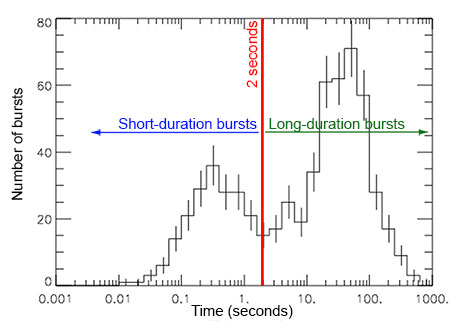
\includegraphics[width=0.5\textwidth]{Figuras/burst_durations_labelled.jpg}
  \caption{Gráfico que muestra la diferencia de tiempo que existe entre GRBs cortos y GRBs largos. Se pueden apreciar 2 picos que marcan la diferencia de duracion entre los GRBs}
  \label{fig:Batse_duration_GRBs}
\end{figure}

El objetivo principal del estudio de los GRBs es analizar las propiedades de los estallidos de los rayos gamma, así como sus progenitores y determinar las propiedades básicas de estos, la fusión de objetos compactos es el modelo progenitor más atractivo. La interacción de flujos de salida relativistas con el medio ambiente que lo rodea produce emisión sincrotrónica que va desde la banda de las ondas de radio a los rayos X, los GRBs son uno de los eventos que más libera energía en el universo, la energía liberada es del orden de $10^{52}$ ergs.

Aunque hay mucha información acerca de los GRBs largos, los cortos son aún un estudio nuevo en el área de astrofísica de altas energías ya que debido a su corta duración son difíciles de estudiar. 
\section{Características de los GRBs}
Muchas de las características de los GRBS ya sean estos largos o cortos, son la duración media que tienen, mientras que en los GRBs largos tienen un promedio de duración de 100 s, los GRBs cortos duran menos de 2 segundos. Los estallidos de Rayos gamma se encuentran a miles de años luz de nuestra galaxia por lo que se puede decir que tienen un orígen cosmologico, mientras los GRBs largos se originan en los centros de las galaxias, los cortos lo hacen lejos de la galaxia donde se originaron y por consecuencia, estos tienen una densidad de ambiente muy bajo. El estudio de los SGRB ha sido muy difícil debido al tiempo de duración que conllevan estos eventos y a la dificultad de asociarlo con galaxias anfitrionas. 

%Las partes principales de los GRBs son la emisión propmt y  afterglow. %Piran2005
 
 
 \begin{figure} %fuente de la imagen:https://astrobites.org/2017/11/13/grb-afterglows-coming-out-of-a-cocoon/
  \centering
    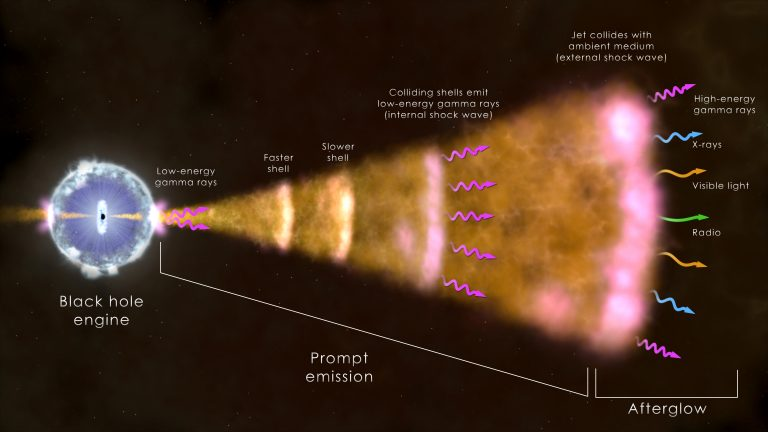
\includegraphics[width=0.5\textwidth]{Figuras/Gamma-ray_burst_by_a_blackhole-768x432.jpg}
  \caption{Diferentes partes de un GRB en general, mostrando las partes más características como el afterflow y la emisión prompt}
  \label{fig:Partes de GRBs}
\end{figure}
 

\subsection{Emisión pronta} %Azzam
La emisión pronta es definido como el periodo de tiempo donde el detector de rayos $\gamma$ detecta una señal sobre el fondo. Estas consisten en fotones de alta energía, no tiene espectro térmico. El espectro térmico es producido por un gas en equilibio térmico. Además, tiene bastantes carterísticas observacionales.

El flujo de energía varia dentro de cientos de Kev. La emisión de las curvas de luz son notoriamente irregulares sobre escalas de tiempo muy pequeñas (ver figura \ref{lightcurve}). %Short gamma-ray bursts: A review; P. D’Avanzo
En los GRBs cortos, su espectro de emisión, se ha encontrado más duro que en los GRBs largos, esto debido a que es una combinación de componentes espectrales duros de baja energía. 

\begin{figure}
\centering %Fuente Zhang
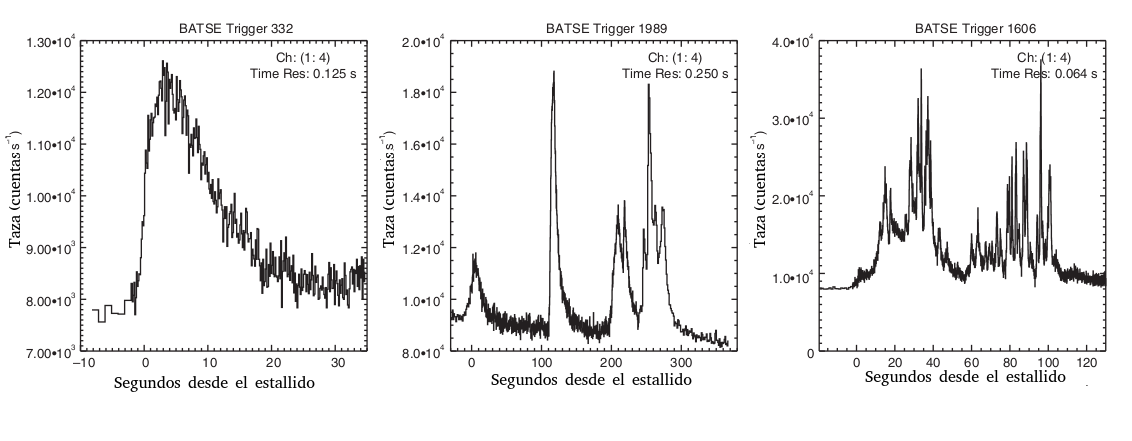
\includegraphics[width=1.0\textwidth]{Figuras/lightcurve_different}
\caption{\label{lightcurve} Diferentes curvas de luz captadas por el detector Batse detectadas en la emisión pronta de los GRBs. Las curvas de luz difieren bastantes unas de otras, mientras que BATSE 332 es un decaimiento exponencial , BATSE Trigger 1989  tiene 2 picos de intensidad. }
\end{figure}
\subsection{Emisión tardía}
La emisión afterglow es despues de la emisión prompt en el cual se pueden detectar otras longitudes de onda como el óptico, radio y los rayos X. %\ref{fig:Partes de GRBs}.
La propiedad de "multiples longitudes de onda", hace una propiedad única de la emisión tardía. Estos cubren un amplio rango de frecuencias, desde las ondas de radio hasta los Tev. El espectro de banda ancha es descrito como una ley de potencias inversa, ya que la fuerza del choque se reduce a medida que la onda expansiva va desacelerando. Con lo que se espera que todas las longitudes de onda de las curvas de luz decaigan como ley de potencias. Entonces la densidad de flujo puede ser representada como:

\begin{equation}
F_{\nu}(t,\nu) \propto t^{-\alpha} \nu^{\beta}
\end{equation}

Donde $\alpha$ y $\beta$ son reales positivos.


 En Mayo y Julio del 2005 datos de eyecciones recopiladas por el satélite \emph{swift} al seguir al seguir al GRB 050509B, descubrieron las primeras fases tardías de los GRBs cortos, tiempo después el satélite HETE-2 junto con el observatorio \emph{chandra} de rayos X siguieron al satélite 050709 el cual localizo la fase tardía en rayos X y despues en la banda óptica, con estos datos recabados de la fase tardía se pudo llegar a que los GRBs cortos tienen una escala de densidad y una energía mas baja que los GRBs largos, tambien se llego a la conclusión de que los GRBs cortos tienen orígenes cosmologicos y que las estrellas masivas no son sus progenitores como en el caso de GRBs cortos.
\subsection{Energía y luminosidad}

%
\section{Características de los GRBs cortos}
Los progenitores de los SGRBs tienen una amplia distribución de tiempo de retraso y su taza es influenciada en parte por la actividad de formación de las estrellas. Las patadas natales pueden ser las causantes de las distancias en las que estos nacen y los sitios de explosión de estos sistemas, la probabilidad para una galaxia de brillo $m$  a ser localizada a una separación $\delta R$ de la posición de un SGRB está dada por 

\begin{equation}
P_{cc} = 1 - \exp ^{- \pi (\delta R)^{2} \sum(\leq m)}
\end{equation}

Donde $\sum(\leq m) = 1.3\cdot 10^{0.33(m-24)-2.44 arcsec ^{-2}}$ son el número de cuentas de la galaxia. Los SGRBs sin galaxias anfitrionas se exhiben cerca galaxias de campo con una baja probabilidad de coincidencia, generalmente las distancias medias de separación del SGRB con su galaxia anfitriona es de $ \frac{\delta R}{r_e} \approx 1.5$ donde $r_e$ es el radio estelar. Otra característica que distingue también a las SGRB es que sus anfitriones tienden a ser mas largos que los anfitriones de los largos.

Los parámetros claves de interes de la emisión pronta y tardia:
\begin{itemize}
\item $E_{\gamma}$: Escala de energía
\item $E_k$: Energía cinética de la onda de choque de la emisión tardía
\item $\theta_j$: El ángulo de apertura del jet
\item $n$: Densidad del medio ambiente
\end{itemize}

El espectro de emisión sincrotrónica (flujo relativista interactuando con el medio circundante) se caracteríza por 3 frecuencias:
\begin{itemize}
\item $\nu_a$: Auto absorción
\item $\nu_m$: Factor mínimo de Lorentz
\item $\nu_c$: enfriamiento sincrotrónico
\end{itemize}

La mayoría de estas frecuencias se encuentran entre 1 $\thicksim$ 10 GHz por lo cual ha sido difícil de detectarlas. La colimación del jet también influye en la taza de los SGRBs y proporciona una restricción adicional al modelo progenitor, la firmatura de la colimación de los destellos de los SGRBs son los llamados "Jet Break" que ocurren al tiempo $t_j$ cuando $\Gamma_j(t_j) = 1/ \theta_j$, esto lidera al cambio de emisión del espectro sincrotrónico

\begin{equation}
F_\nu \propto t^{-1} \longrightarrow F_\nu \propto t^{-p}
\end{equation}

La relación entre el "jet break" y el ángulo de apertura esta dado por:

\begin{equation}
\theta_j = 0.13 \left( \frac{t_{j,d}}{1+z} \right)^{3/8}
\left(\frac{n_0}{E_{52}} \right)^{1/8}
\end{equation}

\section{GRB del 17 de agosto del 2017}
%
\chapter{Teoría}
Para describir un sistema de partículas como un fluido bajo ciertas condiciones uno debe de conocer que el camino libre medio debe de ser mucho mas pequeño que la escala de longitud de las fluctuaciones de las variables macroscópicas.

\begin{equation}
\lambda_{mfp} \ll L
\end{equation}

El tiempo entre las colisiones debe de ser pequeña comparada con la escala del tiempo de los cambios en el fluido
\begin{equation}
t_{c} \ll t_f
\end{equation}
La distancia media entre las partículas tiene que ser mas pequeña que la longitud de escala de las variables macroscópicas

\begin{equation}
l = n^{-1/3} \ll L
\end{equation}



\section{Ecuaciones de la hidrodinámica}

Considerando una serie de elementos de volumen fijos, las ecuaciones que describen el movimiento de un fluido sin considerar efectos viscosos son:

La conservación de masa
\begin{equation} \label{conservación_masa_hidrodinamica}
\dfrac{\partial \rho }{\partial t} + \nabla \cdot \left( \rho \mathbf{u} \right)
\end{equation}

El momento
\begin{equation}  \label{conservacion_momento_hidrodinamica}
\dfrac{\partial \left( \rho \mathbf{u} \right) }{\partial t}+ \nabla \cdot \left( \rho \mathbf{u u} \right) + \nabla p = \mathbf{f_{ext}}
\end{equation}

Ecuación de la energía

\begin{equation} \label{conservacion_energia_hidrodinamica}
\dfrac{\partial E }{\partial t} + \nabla \cdot \left[ \mathbf{u} \left( E+p \right) \right] =G-L+\mathbf{f_{ext} \cdot \mathbf{u}}
\end{equation}

Ecuación de estado
\begin{equation}
E=\frac{1}{2} \rho \mathbf{u}^{2} + \frac{p}{\Gamma - 1}
\end{equation}

Con estas ecuaciones podemos formar una matriz de $5x5$ escritas en coordenadas cartesianas:

\begin{equation} \label{euler_cartesianas}
\dfrac{\partial \mathbf{U}}{\partial t}+\dfrac{\partial \mathbf{F}}{\partial x}+\dfrac{\partial \mathbf{G}}{\partial y}+\dfrac{\partial \mathbf{H}}{\partial z}= \mathbf{S}
\end{equation}

Donde\\
\begin{center}


$\mathbf{U}=
\left(\begin{smallmatrix}
\rho \\
\rho u \\
\rho v \\
\rho w \\
E \\
\end{smallmatrix}\right)
$,
$\mathbf{F} =
\left(\begin{smallmatrix}
\rho u \\
\rho u^{2}+P \\
\rho uv \\
\rho uw \\
u(E+P) \\
\end{smallmatrix}\right)
$,
$\mathbf{G} =
\left(\begin{smallmatrix}
\rho v\\
\rho vu \\
\rho v^{2}+P \\
\rho vw \\
v(E+P) \\
\end{smallmatrix}\right)
$,
$\mathbf{H} =
\left(\begin{smallmatrix}
\rho w\\
\rho wu \\
\rho wv \\
\rho w^{2}+P \\
w(E+P) \\
\end{smallmatrix}\right)
$, 
$\mathbf{S} =
\left(\begin{smallmatrix}
0 \\
f_{x} \\
f_{y} \\
f_{z} \\
G-L+\textbf{f} \cdot \textbf{u} \\
\end{smallmatrix}\right)
$
\end{center}

El término de $\mathbf{U}$ son nuestras variables conservadas, los términos $\mathbf{F}$, $\mathbf{G}$, $\mathbf{H}$ son nuestros fluidos  con velocidades en la dirección $x$, $y$ y $z$ y $\mathbf{S}$ son los términos fuente. Para poder resolver computacionalmente estas ecuaciones diferenciales parciales vamos a utilizar el método de las diferencias finitas y el método de Lax sin considerar tos términos fuente es decir $\mathbf{S}=0$ en el siguiente capitulo si se trataran fuentes particulares.

\section{Hidrodinámica relativista}
En esta parte se añadirá a los códigos que ya hemos generado previamente, las próximas secciones abordara acerca de como cambian nuestras primitivas, como afectan a nuestras variables conservadas y como las podemos desacoplar así como varios ejemplos al cambiar varios valores de nuestros parámetros y de las condiciones iniciales

\subsection{Primitivas}
Las ecuaciones que teníamos para fluidos newtonianos se pueden modificar para hacerlos relativistas. Para esto vamos a partir de 2 ecuaciones importantes que son la ecuación de energía-momento y la ecuación de conservacion de masa:

\begin{equation}\label{Ecuacion_conservación_masa}
\left( \rho u^{\alpha} \right)_{, \alpha} =0
\end{equation}

\begin{equation}\label{Ecuacion_momento_energia}
T_{, \beta}^{\alpha \beta}=0
\end{equation}

De la ecuación \ref{Ecuacion_conservación_masa} tenemos la cuadrivelocidad para un sistema de 3 coordenadas y la velocidad $c=1$ lo podemos ver como $u^{\mu}=\gamma \left( 1, \textbf{v}\right)$ y sustituyendo este resultado (en 2 dimensiones espaciales) tendremos las ecuaciones $u_1$, $F_1$ y $G_1$. Para la ecuación \ref{Ecuacion_momento_energia} podemos escribir el tensor de energía-momento como $T^{\mu \nu} = \rho h u^{\mu} u^{\nu} + Pg^{\mu \nu}$ y usando la métrica de Minkowski

\begin{equation}
\eta_{\alpha \beta}= 
\begin{pmatrix}
 -1 & 0 & 0 & 0 \\
 0 & -1 & 0 & 0 \\
 0 & 0 & -1 & 0 \\
 0 & 0 & 0 & 1 \\
\end{pmatrix}
\end{equation}

Con lo que podemos escribir a $T^{\mu \nu}$ matricialmente como:

\begin{equation}
T^{\mu \nu} =
\begin{pmatrix}
\rho h \gamma^2-P & \rho h \gamma^2 v_{x}  & \rho h \gamma^2 v_{y} & \rho h \gamma^2 v_{z} \\

\rho h \gamma^2 v_{x} & \rho h \gamma^2 v_{x}^{2}+P & \rho h \gamma^2 v_{x}v_{y} &  \rho h \gamma^2 v_{x}v_{z} \\

rho h \gamma^2 v_{y} & \rho h \gamma^2 v_{y}v_{x} & \rho h \gamma^2 v_{y}^{2}+P & \rho h \gamma^2 v_{y}v_{z}\\

\rho h \gamma^2 v_{z} & \rho h \gamma^2 v_{z}v_{x} & \rho h \gamma^2 v_{z}v_{y} & \rho h \gamma^2 v_{z}^2 + P
   
\end{pmatrix}
\end{equation}
Entonces nuestras ecuaciones quedarían de la siguiente manera
\begin{align}
u_{1}& = \rho \gamma \\ 
u_{2}& = \rho v_{x} \gamma^{2} h \\ 
u_{3}& = \rho v_{y} \gamma^{2} h \\ 
u_{4}& = \rho \gamma^{2} h - P 
\end{align}

Donde $\rho$ es la densidad, $\gamma$ es el factor de lorentz, $v_{x}$ y $v_{y}$ son las velocidades de nuestros fluidos (en 2 dimensiones pero se puede extender esto a 3 sin ningún problema), $h$ es la entalpía  y $P$ es la presión. Para los fluidos quedan de la siguiente manera
\begin{align}
F_{1}& = \rho v_{x} \gamma \\ 
F_{2}& = \rho v_{x} v_{x} \gamma^{2} h + P\\ 
F_{3}& = \rho v_{x} v_{y} \gamma^{2} h \\ 
F_{4}& = \rho v_{x} \gamma^{2} h 
\end{align}

\begin{align}
G_{1}& = \rho v_{y} \gamma \\ 
G_{2}& = \rho v_{y} v_{x} \gamma^{2} h \\ 
G_{3}& = \rho v_{y} v_{y} \gamma^{2} h + P\\ 
G_{4}& = \rho v_{y} \gamma^{2} h
\end{align}
\begin{align}
H_{1}& = \rho v_{z} \gamma \\ 
H_{2}& = \rho v_{z} v_{x} \gamma^{2} h \\ 
H_{3}& = \rho v_{z} v_{y} \gamma^{2} h \\ 
H_{4}& = \rho v_{z}^{2} \gamma^{2} h + P
\end{align}



\section{Desacoplamiento de las ecuaciones de la hidrodinámica}

Al final del metodo de las diferencias finitas, obtenemos nuestras variables conservadas (\emph{U}), pero para calcular nuestros flujos de nuevo necesitamos recuperar nuestras primitas, es decir, calcular nuestras variables primitivas $(\rho, \, u, \, v,\, w, \, P )$ en función de nuestras variables conservadas $(u_1, \, u_2, \, u_3, \, u_4, \, u_5)$.

Despejar la densidad es sencillo ya que es directo $u_1= \rho$ por lo tanto:

\begin{equation}\label{primitiva_densidad}
\rho = u_1
\end{equation}

Para las velocidades $u_i=\rho \upsilon$, donde $i=2,3,4$ y $\upsilon=u,v,w$, nos da $\upsilon= u_i/ \rho$ y usando la ecuación \ref{primitiva_densidad} queda:

\begin{equation} \label{primitiva_velocidades}
\upsilon = u_1/u_i
\end{equation}
Para la ecuacion de la energía $u_5=E$ combinando con la ecuacion de estado y la ecuación \ref{primitiva_velocidades} obtenemos
\begin{equation}
P = \left( \Gamma - 1 \right) \left[ u_5 - \frac{u_1 \left( \sum_{i=2}^{4} u_1/u_i \right)^2}{2} \right]
\end{equation}

\section{Desacoplamiento de las ecuaciones de la hidrodinámica relativista}
Para poder desacoplar las ecuaciones, partimos de la relación de las densidades de energía total y del módulo de los momentos

\begin{equation}\label{ecuacion_de_energia}
E=W-p
\end{equation}

\begin{equation}\label{modulos de los momentos}
\abs{m}^2= W^{2}\abs{v}^{2}
\end{equation}

Donde $W=D h \gamma$ y $D=\rho \gamma$. Para evitar errores en el límite no relativista se debe resolver la ecuación conservada restando la densidad de masa a la energía para definir una nueva variable conservada ($E^{'}=E-D$), para las cancelaciones en el límite ultra-relativista basados en $\gamma \abs{v^2}$ que se tiene cuando $\abs{v} \rightarrow 1$, se debe de crear otra variable, que en este caso seria $\abs{u}^2=\gamma \abs{v^2}$ e introduciendo las variables $W^{'}=W-D$. Podemos re-escribir la última ecuación de la siguiente manera

\begin{eqnarray*}
 W^{'}& = &D(h \gamma -1)\\
&=& D\left[ \left(1-\epsilon+ \frac{p}{\rho}\right) \gamma - 1 \right]\\
&=& D \left(\gamma-1 \right) \frac{\gamma+1}{\gamma+1}+\frac{D \gamma }{\rho}\left(\rho \epsilon + p \right)
\end{eqnarray*}

Recordando que $D=\rho \gamma$ y que a partir de la variable introducida $u^{2}$ podemos re-scribir el factor de Lorentz como $\gamma^{2} = 1- u^{2}$

\begin{eqnarray}\label{W_prima}
\nonumber W^{'}&=&\frac{D u^{2}}{\gamma + 1}
+\frac{\rho\gamma \gamma}{ \rho }\left(\rho \epsilon + p \right)\\
&=& \frac{D u^{2}}{\gamma + 1} + \gamma^{2} \chi
\end{eqnarray}

Donde $\chi=\rho \epsilon + p$, derivando con respecto a $W^{'}$ la ecuación \ref{ecuacion_de_energia} queda como
\begin{equation}\label{derivada_E_W}
\dfrac{dE}{dW^{'}}=1-\dfrac{dp}{dW^{'}}
\end{equation}

Nosotros no sabemos como es la expresión $\dfrac{dE}{dW^{'}}$, así que asumiremos que $p=p(\rho, \chi)$ por lo que podemos aplicar la regla de la cadena (para mas detalles consulte)
\begin{equation}\label{cadena}
\dfrac{dp}{dW^{'}}=\dfrac{\partial p}{\partial\chi}\Bigg |_{\rho} \dfrac{d\chi}{dW^{'}} + \dfrac{\partial p}{\partial \rho}\Big |_{\chi} \dfrac{d \rho}{d W^{'}}
\end{equation}

Para calcular $\dfrac{dp}{d\chi}$ tenemos que por ser el caso de un gas ideal
\begin{equation}
h=1+\frac{\Gamma}{\Gamma-1}\frac{p}{\rho}
\end{equation}
Donde $h$ también puede ser escrito como
\begin{equation}
h=1+\epsilon+\frac{p}{\rho}
\end{equation}
Si combinamos estas 2 últimas ecuaciones podemos llegar a que 
\begin{equation}
p(\chi,\rho)=\frac{\Gamma-1}{\Gamma}\chi
\end{equation}

Con lo que al derivar con respecto de $\chi$ nos da como resultado
\begin{eqnarray}\label{der_presion}
& \dfrac{d p}{d \chi}&=\frac{\Gamma-1}{\Gamma}\\ &\dfrac{d p}{d \rho}&= 0
\end{eqnarray}

De la ecuación \ref{W_prima} podemos despejar $\chi$, lo que queda como
\begin{equation}
\chi=\frac{W^{'}}{\gamma}- \frac{D u^{2}}{(1+\gamma)\gamma^{2}}
\end{equation}

Derivando implícitamente la ecuación \ref{W_prima} respecto a $W^{'}$ nos quedaría
\begin{eqnarray*}
W^{'}&=&D\left(\gamma-1 \right) + \chi \gamma^{2}\\%saloto de linea
&=& D\left(\frac{1}{\sqrt{1-\nu^{2}}} -1\right)+\chi \dfrac{1}{1-\nu^{2}} \\%saloto de linea
\dfrac{d W^{'}}{d W^{'}} &=& D \dfrac{d (1-v^2)^{-1/2}}{d W^{'}}+\dfrac{d \chi}{dW^{'}}(1-v^2)^{-1}+\dfrac{d (1-v^2)^{-1} }{d W^{'}}\chi \\  %salto de linea 
1 &=& \frac{D(1-v^2)^{-3/2}}{2} \dfrac{d v^{2}}{d W^{'}}+\dfrac{d \chi}{dW^{'}}(1-v^2)^{-1}+ \chi (1-v^2)^{-2}  \dfrac{d v^{2}}{d W^{'}} \\ %salto de linea
\frac{1}{\gamma ^2} &=& \frac{D \gamma}{2} \dfrac{d v^{2}}{d W^{'}} + \dfrac{d \chi}{dW^{'}} + \chi \gamma^2 \dfrac{d v^2}{dW^{'}} \\ %salto de linea
\end{eqnarray*}

Con lo que al final la ecuación se puede escribir de la siguiente manera

\begin{equation}\label{der_chi}
\dfrac{d \chi}{dW^{'}}=\frac{1}{\gamma^2}-\frac{\gamma}{2}(D-2\gamma \chi) \dfrac{d v^2}{dW^{'}}
\end{equation}

Y para

\begin{equation}\label{der_rho}
\dfrac{d \rho}{d W^{'}}= D \dfrac{d\left(1/ \rho \right) }{d W^{'}} = - \frac{D \gamma}{2}  \dfrac{d v^2}{dW^{'}}
\end{equation}

despejando la ecuación \ref{modulos de los momentos} podemos llegar a escribir el módulo de la velocidad al cuadrado de la siguiente manera
\begin{equation}
\abs{v^{2}} = \frac{\abs{m^{2}}}{W^{'}} 
\end{equation}
Donde $m_i= \rho v_i \gamma h$ para $i=x,y$.

Podemos demostrar que $\dfrac{d \abs{v^2}}{W}=\dfrac{d \abs{v^2}}{W^{'}}$ para esto vamos a partir de de lo siguiente 
\begin{eqnarray*}
\abs{v^2}&=& \abs{m^{2}} \left(W^{'} + D \right)^{-2} \\
\dfrac{d \abs{v^2}}{d W^{'}} &=& \frac{-2 \abs{m}^2}{W^{'}+D^{3}} \\
&=& \frac{2 \abs{m}^2}{W^{3}} \\
&=& \dfrac{d \abs{v^2}}{d W^{'}}
\end{eqnarray*}

Con lo que podemos decir que 

\begin{equation}\label{der_v2}
\dfrac{d\abs{v}^2}{d W^{'} }=-\frac{2 \abs{m}^{2}}{W^{3}}
\end{equation}
Con todo esto ya sabemos cuanto es lo que vale la ecuación \ref{derivada_E_W}, con esto ya podemos usar el método de Newton-Raphson para poder encontrar $W^{'}$.\\

El método de Newton-Raphson es un algoritmo iterativo que se usa para encontrar raíces  de una función real:

\begin{equation}
W^{'(k+1)}=W^{'}-\frac{f(W^{'})}{\dfrac{d f(W^{'})}{d W^{'}}}
\end{equation}

De la ecuación de la energía, podemos utilizarla como a la función a la que queremos encontrar la raíz

\begin{equation} \label{ecuación_f}
f(W^{'})=W^{'}-E^{'}-p
\end{equation}

Donde $E^{'}=W^{'}-p$ y que $\dfrac{d f(W^{'})}{d w} \equiv \dfrac{dE}{dW^{'}}$ dado por la ecuación \ref{derivada_E_W}. Para iniciar el proceso de iteración se tiene que hacer una suposición, para esto, con ayuda de las ecuaciones \ref{ecuacion_de_energia} y \ref{modulos de los momentos} podemos llegar a que la presión es:
%===============================================================================================

\begin{equation} \label{presion_de_newton}
p=\frac{\abs{m}^{2}-W^{2}\abs{v}^{2}+4W^{2}-4EW}{4W}
\end{equation}

Como podemos ver el denominador es una función convexa cuadrática que depende $\abs{v}^{2}$ y $W$ y cumple con que $W$ este fuera del intervalo de las raíces positivas y negativas.

Al denominador de la  ecuación podemos encontrar $W$ ya que $\abs{v}^{2}=1-1/\gamma^{2}$ suponiendo $\gamma \rightarrow \infty$ podemos despejar $W$

\begin{equation}\label{suposicion_de_W}
W=\frac{-(-2E)+\sqrt{(-2E)^{2}-(3)(\abs{m}^{2})}}{3}
\end{equation}

Con esto ya se puede hacer las aproximaciones para obtener $W$, y podemos calcular las siguientes relaciones 
\begin{eqnarray}
\abs{v}^{2} &=& \frac{\abs{m}^{2}}{W^{2}}\label{prim_v2}\\ 
u^{2}&=&\frac{\abs{v}^{2}}{1-\abs{v}^{2}}\label{u2}\\
\gamma &=& \sqrt{1+u^{2}}
\end{eqnarray}
Y las nuevas primitivas.\\

Velocidades:
\begin{eqnarray}
v_{x}&=&\frac{u_{2}}{W}\\
v_{y}&=&\frac{u_{3}}{W}\\
\end{eqnarray}

Densidad de masa 
\begin{equation}
\rho=\frac{D}{\gamma}
\end{equation}

Presión térmica
\begin{eqnarray}
\chi&=&\frac{W-D}{\gamma^{2}}-\frac{D \abs{u}^{2}}{(1+\gamma)\gamma^{2}}\\
p&=&\frac{\Gamma-1}{\Gamma} \chi
\end{eqnarray}



\section{Diferencias finitas} \label{sec:Diferencias_finitas}
Si tenemos una función $f(x)$ lo suficientemente diferenciable la podemos aproximar por el Teorema de Taylor  en la vecindad de un punto $x_0+\Delta x$ entonces si conocemos todas sus $n$ derivadas de la función $f(x)$ en el punro $x_0$ podemos aproximar de la siguiente manera

\begin{equation}\label{Serie_Taylor}
f\left( x_0 + \Delta x\right) = f\left( x_0 \right)+
\sum_n \frac{\left( \Delta x \right) ^2}{k!}f^{(k)} \left(x_0
\right)
\end{equation}

Si truncamos la serie de Taylor y quitamos los términos de segundo orden podemos escribir la ecuación \ref{Serie_Taylor} como:

\begin{equation}
f\left( x_0 + \Delta x \right) = f(x_0) - \Delta x f^{(1)} (x_0) + O \left( \Delta x \right)
\end{equation}

Despejando $f(x_0)$ queda lo que se conoce como diferrencia finita hacia adelante
\begin{equation}\label{fwd}
f_{fwd}^{'}=\frac{f\left(x + \Delta x \right) - f(x) }{\Delta x}=\frac{f_{i+1}-f_{i}}{\Delta x}
\end{equation}

Tambien se puede hacer en el entorno $x_0- \Delta x$ y siguiendo los mismos pasos anteriores llegamos a lo que se le conoce como diferencia finita hacia atras.



\begin{equation}\label{bwd}
f_{back}^{'}=\frac{f\left(x \right) - f(x - \Delta x) }{\Delta x}=\frac{f_{i}-f_{i-1}}{\Delta x}
\end{equation}

Si obtenemos el promedio de las ecuaciones \ref{fwd} y \ref{bwd} obtenemos la central:

\begin{equation} \label{Centrada}
f_{central}^{'}=\frac{f\left(x + \Delta x\right) - f(x - \Delta x) }{2\Delta x}=\frac{f_{i+1}-f_{i-1}}{2 \Delta x}
\end{equation}



\subsection{Lax-Friederich}

Si consideramos la siguiente ecuación diferencial parcial

\begin{equation} \label{ecu_conser}
u_t+ f\left(u \right)_t=0
\end{equation}

Un método conservativo para resolver este tipo de ecuación diferencial es 

\begin{equation}\label{esquema conservativo}
u_i^{n+1} = u_i^{n} -\frac{\Delta t}{\Delta x} \left(f_{i-\frac{1}{2}} - f_{i+\frac{1}{2}}\right)
\end{equation}



Si hacemos la siguiente elección de flujo 

\begin{equation}
f_{i+\frac{1}{2}} = f_{i+\frac{1}{2}} \left(
u_{i} , u_{i+1}\right) =\frac{1}{2} \left(f_{i} + f_{i+1} \right) 
\end{equation}

Y para 

\begin{equation}
f_{i-\frac{1}{2}} = f_{i-\frac{1}{2}} \left(
u_{i} , u_{i-1}\right) =\frac{1}{2} \left(f_{i} - f_{i-1} \right) 
\end{equation}

Y lo sustituimos en la ecuación \ref{esquema conservativo} nos queda el siguiente resultado

\begin{equation}\label{ec_inestable}
u_i^{n+1} = u_i^{n} + \frac{1}{2}\frac{\Delta t}{\Delta x} \left(f_{i+1} - f_{i-1} \right)
\end{equation}

Pero esta solución es inestable, por el primer término del lado derecho de la ecuación, para hacerlo estable  Peter Lax y Kurt O. Friedrichs sustituyerón este término por $(u_{i+1}^n-u_{i-1}^n)$  por lo que podemos reescribir la ecuación \ref{ec_inestable} como

\begin{equation}\label{ec_estable}
u_i^{n+1} =(u_{i+1}^n-u_{i-1}^n) + \frac{1}{2}\frac{\Delta t}{\Delta x} \left(f_{i+1} - f_{i-1} \right)
\end{equation}


\subsection{HLL}

	Otro método para resolver las ecuaciones de la hidrodinámica es usar el método de Harten-Van-Leer. Definiendo el flujo numérico intercelda de Gudonov

\begin{equation}
F_{i+\frac{1}{2}}=F \left( U_{i+\frac{1}{2}} \right)
\end{equation}

Para el cual $U_{i+\frac{1}{2}}(0)$ tiene la misma solución para $U_{i+\frac{1}{2}}(x/t)$ con lo que el problema de Riemann se reduce a :

\begin{equation} \label{Ecuacion_discreta_conservada}
\begin{array}{ll}
U_t + F \left( U \right)_x = 0 \\
U \left(x,0 \right) = 
\left\lbrace
\begin{array}{rr}
U_L \quad \textup{si} \quad x<0  \\
U_R \quad \textup{si} \quad x>0
\end{array}
\right.
\end{array}
\end{equation}

\begin{figure} %fuente de la imagen:libro del toro/
  \centering
    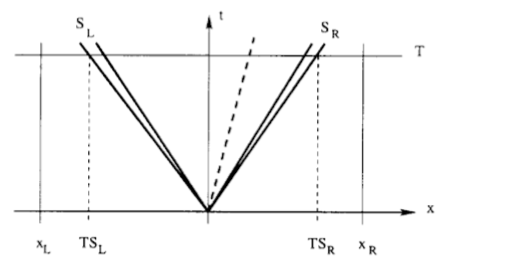
\includegraphics[width=0.5\textwidth]{Figuras/HLL_onda.png}
  \caption{Plano x-t que muestra que muestra un volumen definido}
  \label{fig:Plano x_t}
\end{figure}

Si consideramos un control de volumen $\left[x_L, x_R \right]\times \left[ 0 , T \right]$, tales que $x_L \leq TS_L$ y $x_R \geq TS_R$ (ver figura \ref{fig:Plano x_t}) donde $S_L$ y $S_R$ son las velocidades de las ondas mas rápidas de los estados iniciales $U_L$ y $U_R$ respectivamente y $T$ es un tiempo definido. Si usamos la forma integral de la ecuacion \ref{Ecuacion_discreta_conservada} en nuestro volumen definido $\left[x_L, x_R \right]\times \left[ 0 , T \right]$

\begin{equation*}\label{Forma_integral_conservadas}
\int_{x_L}^{x_R} \left[ U\left( x, T \right) -
 U\left( x, 0 \right) \right] dx = 
 \int_{0}^{T} \left[ F \left(U\left( x_L, t \right) \right) -
 F \left(U\left( x_R, t \right) \right) \right] dt 
\end{equation*}
Entonces
\begin{equation}\label{integral_consistencia}
\int_{x_L}^{x_R} U\left( x, T \right) dx =\int_{x_L}^{x_R} U\left( x, 0 \right) dx+
\int_{0}^{T}  F \left(U\left( x_L, t \right) \right)dt -
\int_{0}^{T}  F \left(U\left( x_R, t \right) \right) dt
\end{equation}

Usando las condiciones de la ecuación \ref{Ecuacion_discreta_conservada} podemos evualuar la integral

\begin{equation*}
\int_{x_L}^{x_R} U\left( x, T \right) dx = 
x_R U_R -x_L U_L+T F_L-T F_R
\end{equation*}
Donde $F_L = F \left( U_L \right)$ y $F_R = F \left( U_R \right)$, entonces

\begin{equation}\label{Condición_de_consistencia}
\int_{x_L}^{x_R} U\left( x, T \right) dx = 
x_R U_R -x_L U_L+T \left( F_L- F_R \right)
\end{equation}

Si separamos ahora la ecuación \ref{integral_consistencia} en 3 integrales de la siguiente manera:

\begin{equation}
\int_{x_L}^{x_R} U\left( x, T \right) dx = 
\int_{x_L}^{T S_L} U \left(x, T \right)dx+
\int_{T S_L}^{T S_R} U \left(x, T \right)dx+
\int_{T S_R}^{x_R} U \left(x, T \right)dx
\end{equation}

Si ahora evualuamos el tercer y el primer término en el lado derecho, obtenemos:

\begin{equation}\label{condicion_consistencia_2}
\int_{x_L}^{x_R} U\left( x, T \right) dx =
\int_{T S_L}^{T S_R} U \left(x, T \right)dx+
\left( T S_L - x_L \right) U_L+
\left( x_L - T S_R \right) U_R
\end{equation}

Si combinamos la ecuación \ref{Condición_de_consistencia} y 
\ref{condicion_consistencia_2}

\begin{equation*}
x_R U_R -x_L U_L+T \left( F_L- F_R \right) =
\int_{T S_L}^{T S_R} U \left(x, T \right)dx+
\left( T S_L - x_L \right) U_L+
\left( x_L - T S_R \right) U_R
\end{equation*}

Entonces 

\begin{equation*}
\int_{T S_L}^{T S_R} U \left(x, T \right)dx=
\left( T S_L - x_L \right) U_L+ x_L U_L +
\left( x_L - T S_R \right) U_R-x_R U_R -
T \left( F_L- F_R \right)
\end{equation*}

Con lo que al final nos queda

\begin{equation} \label{ull_sin_promedio}
\int_{T S_L}^{T S_R} U \left(x, T \right)dx=
T \left( S_R U_R - S_L U_L + F_L - F_R \right)
\end{equation}

Si dividimos la ecuación \ref{ull_sin_promedio} por la diferencia de las velocidades maximas de las señales de las ondas, obtenemos el promedio de la funcion que esta entre las velocidades de la onda, entonces

\begin{equation}
\frac{1}{T \left( S_R -S_L \right)}\int_{T S_L}^{T S_R} U \left(x, T \right)dx =
\frac{S_R U_R - S_L U_L + F_L - F_R}{S_R - S_L}
\end{equation}

Si conocemos las velocidades de la onda podemos escribir la ecuación como 

\begin{equation}\label{u_hll}
U^{hll} = \frac{S_R U_R - S_L U_L + F_L - F_R}{S_R - S_L}
\end{equation}

Ahora si aplicamos la forma integral ( como en el caso de la ecuación \ref{Condición_de_consistencia}) a lado izquierdo de nustro plano obtenemos lo siguiente

\begin{equation}
\int_{T S_L}^{0} U\left( x, T \right) dx = 
-T S_L U_L+T \left( F_L- F_{0L} \right)
\end{equation}
Donde $F_{0L}$ es el flujo a lo largo del eje $t$. Si despejamos $F_{0L}$, nos queda lo siguiente

\begin{equation}\label{ec F_0L}
F_{0L} = F_L - S_L U_L + \frac{1}{T}  \int_{T S_L}^{0} U\left( x, T \right) dx
\end{equation}

Esta última ecuación nos servira para calcular los flujos usando el método de Harteen-Van-Leer, el cual dividian el plano en tres espacios:

\begin{figure} %fuente de la imagen:libro del toro/
  \centering
    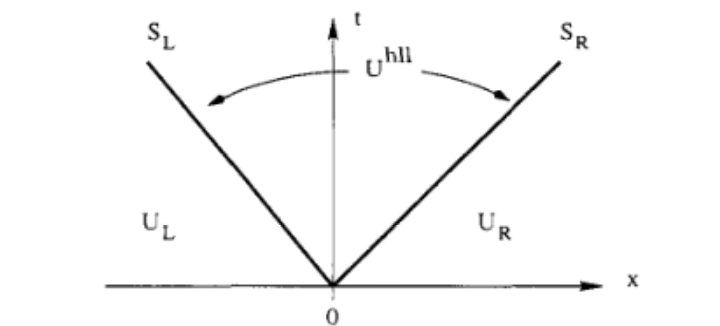
\includegraphics[width=0.5\textwidth]{Figuras/HLL.png}
  \caption{Aproximación de 3 estados distintos en el plano x-t, en el cual se trata de calcular los flujos en la región $U^{hll}$ limitados por las velocidades de señal de la onda}
  \label{fig:HLL}
\end{figure}

\begin{equation}
U \left(x,t \right) = 
\left\lbrace
\begin{array}{rr}
U_L \quad \textup{si} \quad \frac{x}{t}< S_L  \\
U_{hll} \quad \textup{si} \quad S_L< \frac{x}{t} <S_R \\
U_R \quad \textup{si} \quad  \frac{x}{t} > S_R
\end{array}
\right.
\end{equation}

Los flujos $F_R$ y $F_L$ pueden ser calculados directamente ya que solo dependen de $U_R$ y $U_L$ respectivamente pero $F_{hll} \neq F \left( U_{hll} \right)$, asi que resolvemos la integral de la ecuación \ref{ec F_0L} para asi obtener el flujo a traves del eje t

\begin{equation*}
F_{hll} = F_L -S_L U_L+ \frac{1}{T}U_{hll}\left(0- TS_L\right)
\end{equation*}

Entonces
\begin{equation}\label{f_hll 1}
F_{hll} = F_L +S_L \left( U_{hll} -U_L \right)
\end{equation}

Si sustituimos \ref{u_hll} en \ref{f_hll 1} obtenemos:

\begin{equation*}
F_{hll} = F_L +S_L \left( \frac{S_R U_R - S_L U_L + F_L - F_R}{S_R - S_L} -U_L \right)
\end{equation*}
Entonces
\begin{equation*}
F_{hll} = \frac{F_L S_R -F_L S_L+S_L S_R U_R-S_L^2 U_L+S_L  F_L- S_L F_R-S_R S_L U_L + S_L^2 U_L}{S_R-S_L}
\end{equation*}

Eliminando términos semejantes queda
\begin{equation}
F_{hll} = \frac{S_R F_L -S_L F_R + S_L S_R \left(U_R-U_L \right)}{S_R -S_L}
\end{equation}

Con lo que el flujo intermedio de la celda de Gudonov esta dado por:

\begin{equation}
F_{i+\frac{1}{2}}^{hll} = 
\left\lbrace
\begin{array}{rr}
F_L \quad \textup{si} \quad 0 \leq S_L  \\
\frac{S_R F_L -S_L F_R + S_L S_R \left(U_R-U_L \right)}{S_R -S_L} \quad \textup{si} \quad S_L \leq 0 \leq S_R \\
F_R \quad \textup{si} \quad  0 \geq  S_R
\end{array}
\right.
\end{equation}


%\section{Hidrodinámica con fuentes}

%=======================================================================================
%======================================================================================
\chapter{Verificación del código}

En este capítulo se van a realizar algunas pruebas de la funcionalidad de mi código, el objetivo de esto, es tener una idea de cual método, ya sea Lax o HLL, es mejor para la ejecución de los jets.

\section{Onda de choque} %Shock Wave and High Pressure Phenomena) Isabelle Sochet (eds.
La onda de choque se produce por la liberación rápida de energía comprimida dentro de un volumen de radio $R$. Esta explosión divide a nuestro dominio en 2 zonas distintas como se muestra en la figura \ref{fig:onda_choque_example}. La zona I, estará determinado por la densidad, presión, y velocidades del medio ambiente ($\rho_m, \, P_m\, v_{x_m}, \, v_{y_m}$, respectivamente). La zona II (i.e. dentro de la onda de choque), se produce al depositar una densidad de energía $E_{in}$ dentro de una región definida por un radio interno ($R_{in}$) en reposo. Para ver más detalles véase el cuadro \ref{fig:onda_choque_example}.

\begin{table}[htbp]\label{Tabla_parametros}
\begin{center}
\begin{tabular}{|c|c|c|}
\hline 
\textbf{Parámetro} & \textbf{Descripción} & \textbf{valor} \\ 
\hline 
$R_{in}$ & Radio interno de la onda expansiva & 0.2 [cm] \\ 
\hline 
$\rho_{in}$ &  Densidad interna de la onda expansiva & 5.0 [$\mathrm{g} / \mathrm{cm}^3$] \\ 
\hline 
$\rho_{out}$ &  Densidad del medio  & 1.0 [$\mathrm{g} / \mathrm{cm}^3$] \\
\hline 
$P_{int}$ & Presión interna de la onda expansiva & 10.0 [$\mathrm{g}  /  \mathrm{cm}\cdot \mathrm{s}^2$]\\ 
\hline 
$P_{out}$ &  Presión del medio  & 0.1 [$\mathrm{g}  /  \mathrm{cm}\cdot \mathrm{s}^2$] \\ 
\hline 
$v_{x_{int}}$ & Velocidad interna en el eje x de la onda expansiva & 0.0 [$\mathrm{cm}/\mathrm{s}$]\\ 
\hline 
$v_{y_{int}}$ & Velocidad interna en el eje y de la onda expansiva & 0.0 [$\mathrm{cm}/\mathrm{s}$]\\ 
\hline 
$v_{x_{out}}$ & Velocidad en el eje x del medio & 0.0 [$\mathrm{cm}/\mathrm{s}$] \\
\hline 
$v_{y_{out}}$ & Velocidad en el eje y del medio & 0.0 [$\mathrm{cm}/\mathrm{s}$]\\ 
\hline 
Co & Número de Courant & 0.7 \\ 
\hline 
\end{tabular}
\caption{Parámetros que se utilizarán en las siguientes pruebas que se van a realizar para la onda de choque, estos valores son para fluidos no relativistas.}
\end{center}
\end{table}

La $E_{in}$ de la onda de choque está determinada por la $\rho_{in}$, $P_{in}$, y $v_{x_{in}}$ y $v_{y_{in}}$ ya que es la suma de la energía cinética más la energía térmica
$E_{in} = {\frac{1}{2}} \rho_{in} v_{in}^2 + {\frac{P_{in}}{\Gamma -1 }}$).
Dado que la zona II está en reposo $v_{x_{in}}=0$ y $v_{y_{in}}=0$, se tiene:
$E_{in} = {\frac{P_{in}}{\Gamma -1 }}$).
Cabe señalar que los valores de la densidad y presión del medio ambiente tendrán valores mas bajos que sus respectivos de la onda de choque. 

\begin{figure}[H]
\centering
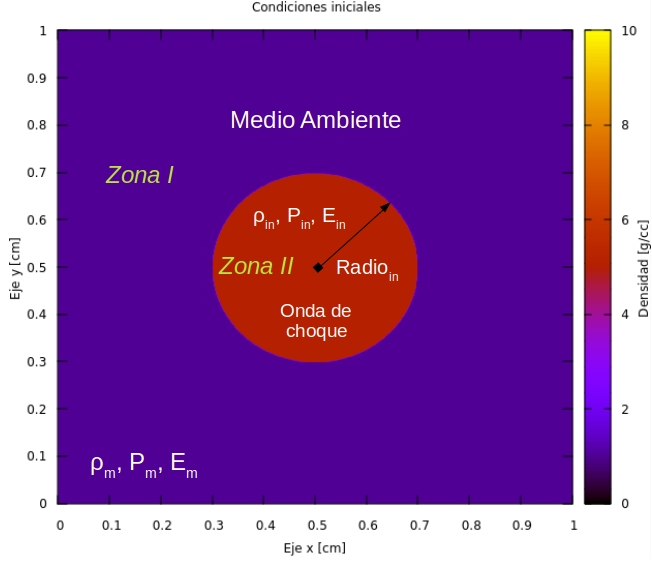
\includegraphics[width=0.6\textwidth]{./Figuras/Pruebas/Prueba_onda_choque/prueba_example}
\caption{\label{fig:onda_choque_example}La zona I (medio ambiente), se caracterizará por tener valores de densidad, presión y velocidades ($\rho_m, \, P_m \, v_{x_m}, \, v_{y_m}$, respectivamente) mostrados en el cuadro \ref{Tabla_parametros}. La zona II (onda de choque) se produce al depositar una energía ($E_{in}$) y una presión ($P_{in}$) dentro de un círculo (con $R_{in}$).}
\end{figure}

La onda de choque se dejó evolucionar con el paso del tiempo, y se analizó la interacción que hay entre las zonas I y II. En específico, se siguió la evolución de una onda de choque con una velocidad de expansión muy por debajo de la velocidad de la luz (denominado como caso newtoniano), y además la evolución de una onda de choque cuya velocidad de expansión estaba cercana a la velocidad de la luz (caso relativista). Cabe señalar que en ambos casos se siguieron los cambios que se produjeron utilizando los método numéricos de Lax y el de HLL (véase la Sección \ref{sec:Diferencias_finitas} para mayor información). La condición a la frontera utilizada en todos los bordes fue la de \emph{outflow}\footnote{Para ver más detalles acerca de esta frontera y/o de otro tipo de fronteras veáse el apéndice \ref{aped.B}}. 


%tiempo = 0.5 s
%lapso = tiempo/20



\subsection{Caso newtoniano} 
%\subsubsection{Lax} \label{subsec: Prueba Lax}
%Como primeras pruebas se realiza: explicas la 3.2, y además se llevó a cabó (explicas la figura 3.5).

%Las dos primeras pruebas: 

%1. Newtoniano + Lax + onda choque centrada 2. Newtoniano + Lax + onda choque borde

Las siguientes pruebas fueron usando el método de Lax, usando las ecuaciones relativistas con la constante de relación específica $\Gamma = 3/4$, así como las newtoniana $\Gamma = 5/3$. La descripción del fenómeno es de una onda expansiva sobre un medio constante (ver figura \ref{fig:onda_choque_example}) con una densidad de energía de $E = 0.15 \, \mathrm{erg} \cdot \mathrm{cm}^{-3}$, densidad $\rho = 1 \, \mathrm{g} \cdot \mathrm{cm}^{-3}$ , velocidades $v = 0 \, \mathrm{cm} \cdot \mathrm{s}^{-1}$ y una presión $P=0.1 \, \mathrm{erg} \cdot \mathrm{cm}^{-3} $. La simulación es sobre un dominio de 0 a 1 cm sobre el eje \emph{x} y de 0 a 1 cm sobre el eje \emph{y}, con una resolución de 500x500 pixeles\footnote{Los píxeles de nuestra malla miden $l_x\cdot 500^{-1} = l_y\cdot 500^{-1}  = 1 \, \mathrm{cm} \cdot 500^{-1} = 0.005 \, \mathrm{cm}$} al tiempo $t=0 \, \mathrm{s}$  y en la onda interna. Su valor de la densidad es de $\rho=5 \, \mathrm{g} \cdot \mathrm{cm}^{-3}$, su velocidad interna será la misma que la del ambiente, la presión interna de la onda $P=10 \, \mathrm{erg} \cdot \mathrm{cm}^{-3} $ y una densidad de energía interna $E = 3.75 \, \mathrm{erg} \cdot \mathrm{cm}^{-3}$. La onda de choque esta centrada en el punto $(x,y) = (0.5, 0.5) \, \mathrm{cm}$, y se correrá en el intervalo de tiempo $t \in \left[ 0 , 0.5 \right]$ s.
%%===================IMAGE_LAX_CENTRADO_T=0===============================
%\begin{figure}[H]
%\centering
%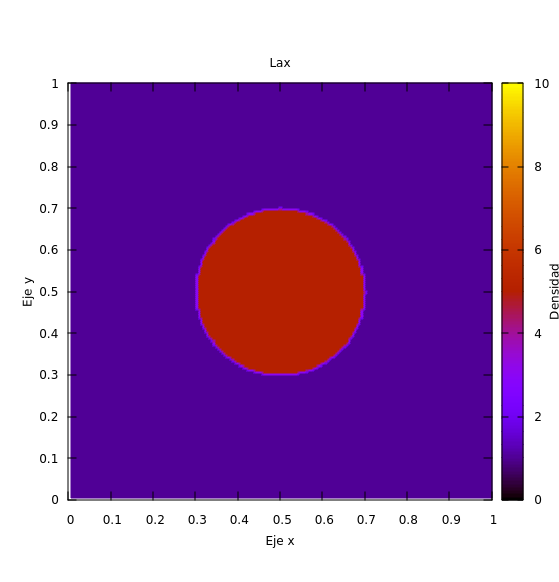
\includegraphics[width=0.5\textwidth]{./Figuras/Pruebas/Prueba_onda_choque/onda_choque1_t_0}
%\caption{Condición inicial ($t = 0$) de una onda de choque (con $\rho_{in}=5.0, \, v_{x_{in}}=v_{y_{in}}=0.0, \, P_{in}=10.0$ y $E_{in}=3.75$), de radio interno $R_{in} = 0.2$ cm. que se va a expandir sobre un medio (con $\rho_{out}=1.0$  y $ P_{out}=0.1$) estático. Véase el Cuadro \ref{Tabla_parametros} para más detalles.} \label{fig:onda_choque1_t_0}
%\end{figure}
%%===================IMAGE_LAX_CENTRADO_T=0===============================

La evolución para la onda de choque newtoniano muestra una expansión de la onda simétrica. El radio de la onda al tiempo inicial fue de $r=0.2$ cm. A $t=0.05$ s la onda se expandió a un radio de $r=0.3$~cm mientras que para el tiempo $t=0.10$ s se expandió a un radio de $r=0.38$~cm. Debido a lo anterior, la velocidad de expansión de la onda fue de $v = 2.0 \, \mathrm{cm} \cdot \mathrm{s}^{-1}$ y $v = 1.8 \, \mathrm{cm} \cdot \mathrm{s}^{-1}$, respectivamente.% FALTA MENCIONAR A FORWARD SHOCK Y LA REVERSE SHOCK.. y por ende el HUECO (ver figura \ref{fig:Lax-newtoniano-prueba1}). ADMÄS FALTA MENCIONAR QUE LA PARTE CENTRAL SE DIFUMINA... LO CUAL ES ESPERABLE DEBIDO A LA VISCOSIDAD NUMERICA.


%===================IMAGE_LAX_CENTRADO_EVOLUCION===============================
\begin{figure}[H]
\centering
\subfigure[$t = 0.05$ s]{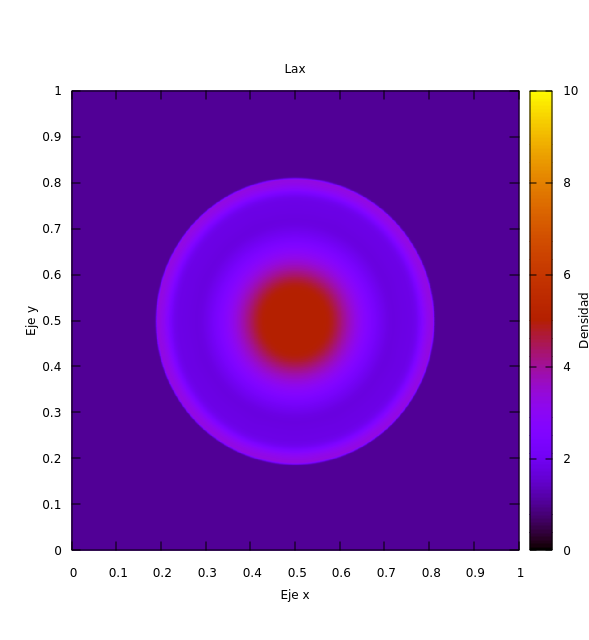
\includegraphics[scale = 0.55]{./Figuras/Pruebas/Prueba_onda_choque/Lax/Lax-sedov3}}
\subfigure[$t = 0.1$ s]{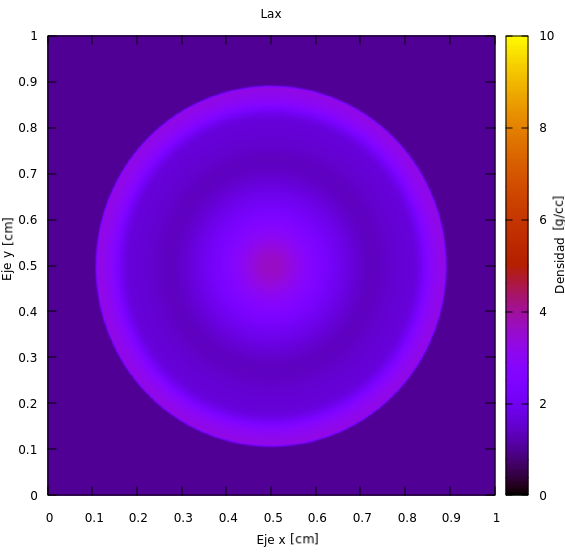
\includegraphics[scale = 0.55]{./Figuras/Pruebas/Prueba_onda_choque/Lax/Lax-sedov5}}
\caption{\label{fig:Lax-newtoniano_sedov-3-5}Evolución de la onda de choque mostrada en la figura \ref{fig:onda_choque_example} usando el método de Lax newtoniano. En el panel a) se muestra la onda de choque a t=0.05s, mientras que en el panel b) se muestra para t=0.10 s. En la figura \ref{fig:Lax-newtoniano-prueba1-analisis} se analizará más a fondo las partes que se forman al desarrollarse dicha onda.}
\end{figure}
%===================IMAGE_LAX_CENTRADO_EVOLUCION===============================


Cuando la onda se empieza a expandir por el medio constante, aparecen 4 áreas distintas que interactuan entre nuestro medio ambiente y la onda. El área 1 (ver figura \ref{fig:Lax-newtoniano-prueba1-analisis}) es el material al cual la onda no ha tocado. En el área 2, se muestra una onda que va chocando con el material del medio ambiente, a esta onda la llamaremos \emph{forward shock}\footnote{La palabra \emph{forward shock} viene del inglés y la podemos interpretar como choque hacia adelante. }. El área 3 presenta el material chocado con el mismo centro de la onda, esta se caracteriza por ir en reversa y llamaremos \emph{reverse shock}\footnote{La palabra \emph{reverse shock} viene del inglés y la podemos traducir como choque hacia atras}, el material contra el cual aún no ha chocado esta onda es el área 5. La separación que hay entre estas 2 ondas vas creando un vacio que se ve difuminado, esto debido a la viscosidad que presenta nuestro resolvedor de Riemann.


%===================IMAGE_LAX_CENTRADO_EVOLUCION_ANALISIS===============================
\begin{figure}[H] 
\centering
\subfigure[$t = 0.05$ s]{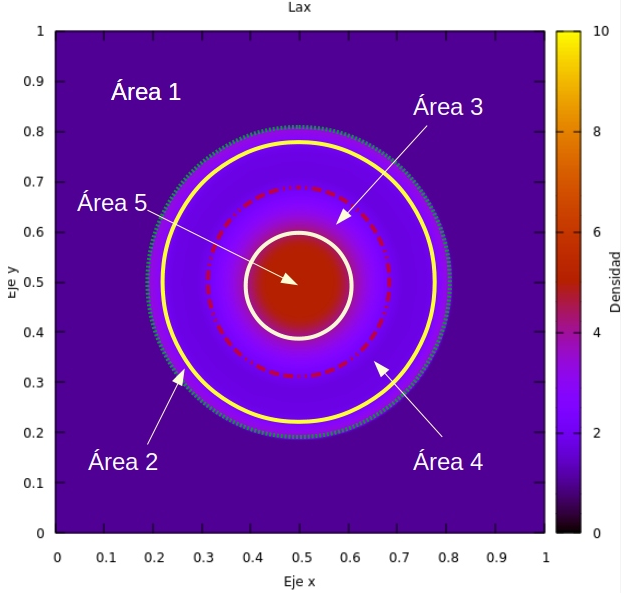
\includegraphics[scale = 0.595]{./Figuras/Pruebas/Prueba_onda_choque/Lax/Lax-sedov3-analisis}}
\subfigure[$t = 0.1$ s]{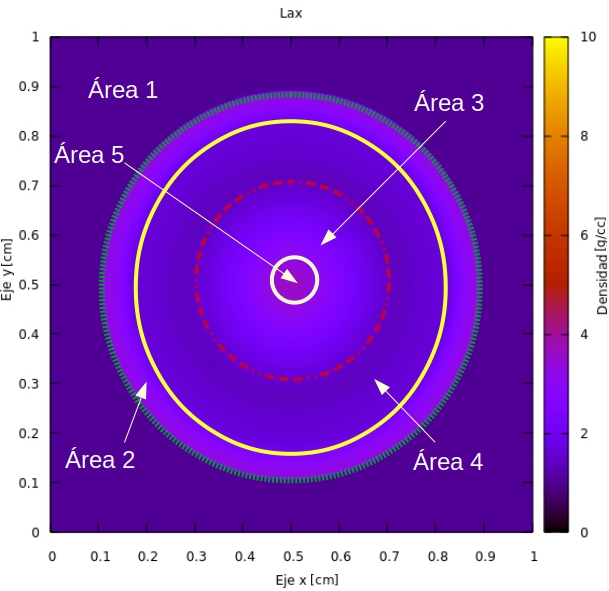
\includegraphics[scale = 0.6]{./Figuras/Pruebas/Prueba_onda_choque/Lax/Lax-sedov5-analisis}}
\caption{\label{fig:Lax-newtoniano-prueba1-analisis}En la evolución de la onda usando el método de Lax, podemos encontrar 4 áreas distintas. El área 1 la identificaremos como el material que no ha sido chocado todavía por nuestra onda. El área 2 será el material que es chocado por nuestra onda, esta onda que se llama \emph{forward shock}. En el área 3 podemos ver una onda que va contra si misma que es la \emph{reverse shock}, esta onda arrastra el interior de la onda, va en sentido contrario a la \emph{forward shock}, el material que esta onda aun no ha chocado es al área 5 y el área 4 es el vacío que se va formando cuando se separan la \emph{forward shock} y \emph{reverse shock}.} 
\end{figure}
%===================IMAGE_LAX_CENTRADO_EVOLUCION_ANALISIS===============================


La segunda prueba consiste en realizar el mismo proceso descrito anteriormente de la onda de choque resuelta con el método de Lax pero, ubicando a la onda de choque en una esquina para poder analizar como se comporta con las condiciones a la frontera. El centro de la nueva prueba se colocó en las coordenadas $(x, y) = (0.25, 0.75)$ [cm]. Cabe señalar que las condiciones a la fronteras tienen la configuración de \textit{outflow}\footnote{Para este y otros tipos de frontera vea el apéndice \ref{aped.B}}.

%===================IMAGE_LAX_NO_CENTRADO_T=0===============================
\begin{figure}[H] \label{fig:onda_choque2_t_0}
\centering
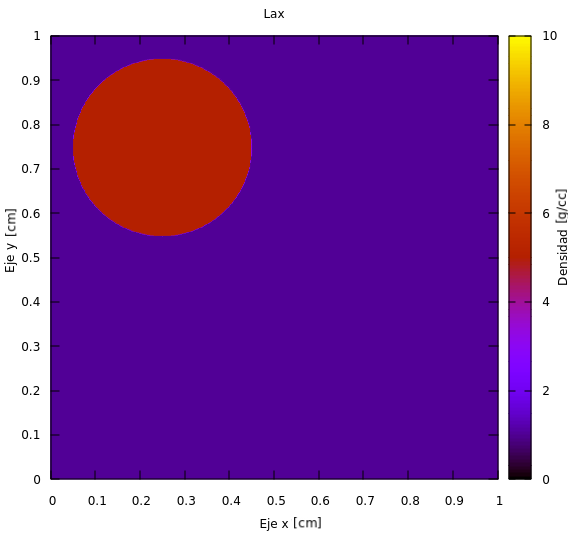
\includegraphics[width=0.6\textwidth]{./Figuras/Pruebas/Prueba_onda_choque/onda_choque2_t_0}
\caption{Condición inicial de la prueba número 2 para el resolvedor Lax newtoniano. En esta prueba se tiene la misma condición inicial que la mostrada en la figura \ref{fig:onda_choque_example}, pero con las coordenadas de la onda de choque ubicadas en $(x, y) = (0.25, 0.75)$ [cm]. Esto con la finalidad de mostrar que sin importar donde se coloquen la onda de choque, esta se comportará de igual manera que si estuviera centrado.} 
\end{figure}
%===================IMAGE_LAX_NO_CENTRADO_T=0===============================


%LAS FRONTERAS NO METEN RUIDO. Y LA EVOLUCIÓN ES CONSISTENTE CON LOS RESULTADOS DE ANTES, Y POR ENDE ESTA BIEN. 
Al evolucionar la onda de choque en la figura \ref{fig:Lax-prueba2_no_centrado},  esta no muestra ninguna anomalía en las fronteras (ver apéndice \ref{aped.B}) y puedo concluir que las condiciones a la frontera no introducen errores numéricos para el caso newtoniano y usando Lax, ya que tiene el mismo comportamiento que de la onda centrada. El radio al tiempo $t = 0.07$ s es $r = 0.34$ cm y su velocidad es $v = 2 \, \mathrm{cm}/\mathrm{s}$ y para el tiempo $t = 0.14$ s el radio $r = 0.42$ y su velocidad $v = 1.83 \, \mathrm{cm}/\mathrm{s}$. Con lo que podemos observar que tiene las mismas particularidades que la onda mostrada en la figura \ref{fig:Lax-newtoniano_sedov-3-5}.


%===================IMAGE_LAX_NO_CENTRADO_EVOLUCION===============================
\begin{figure}[H]
\centering
\subfigure[]{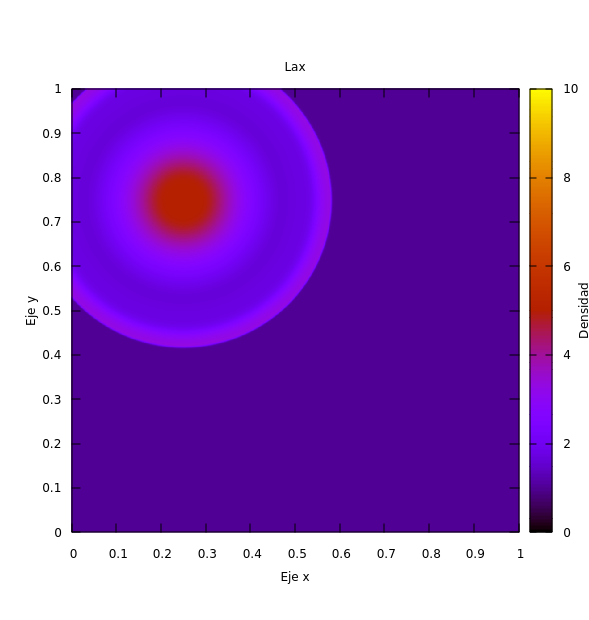
\includegraphics[scale = 0.46]{./Figuras/Pruebas/Prueba_onda_choque/Lax/Lax-sedov2_07}}
\subfigure[]{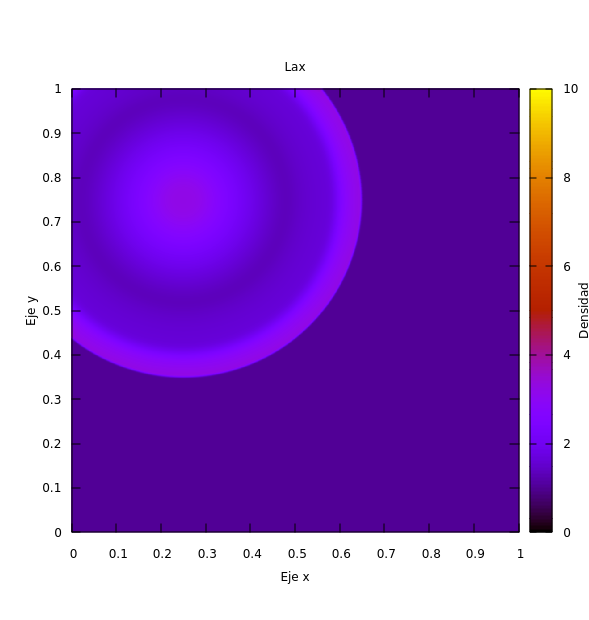
\includegraphics[scale = 0.5]{./Figuras/Pruebas/Prueba_onda_choque/Lax/Lax-sedov2_12}}
\caption{\label{fig:Lax-prueba2_no_centrado}Evolución de la onda de choque mostrada en la Figura \ref{fig:onda_choque2_t_0} usando el método de Lax no relativista. En el panel a) se muestra la onda de choque a t=0.07s, mientras que en el panel b) se muestra para t=0.12s. Al evolucionar la onda se observa que al pasar la frontera no hay ruido o errores y que la velocidad asi como el radio son los mismos que en la onda centrada.} 
\end{figure}
%===================IMAGE_LAX_NO_CENTRADO_EVOLUCION===============================

En la figura \ref{fig:Lax-prueba2_no_centrado-analisis}, al salir de nuestro dominio, la onda sigue conservando su forma y las áreas que habiamos visto en la figura \ref{fig:Lax-newtoniano-prueba1-analisis}. El aspecto de la onda no se deforma a pesar de que se sale del dominio computacional.

%===================IMAGE_LAX_NO_CENTRADO_EVOLUCION_ANALISIS===============================
\begin{figure}[H]
\centering
\subfigure[]{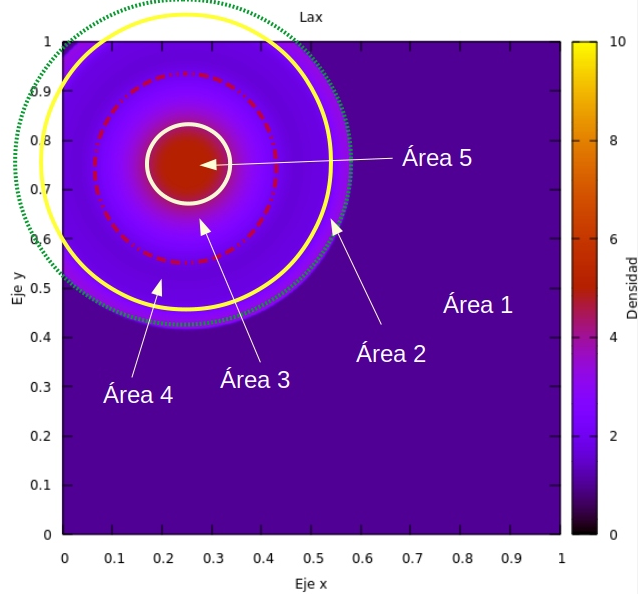
\includegraphics[scale = 0.5]{./Figuras/Pruebas/Prueba_onda_choque/Lax/Lax-sedov2_07-analisis}}
\subfigure[]{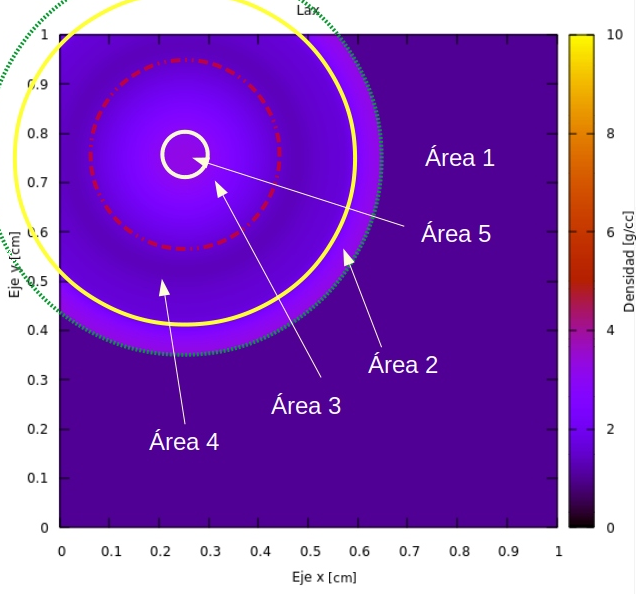
\includegraphics[scale = 0.5]{./Figuras/Pruebas/Prueba_onda_choque/Lax/Lax-sedov2_12-analisis}}
\caption{\label{fig:Lax-prueba2_no_centrado-analisis}Al igual que en la figura \ref{fig:Lax-newtoniano-prueba1-analisis}, la onda presenta 5 áreas descritas, y estas se vuelven más grandes con el paso del tiempo. En el área 4 se puede ver la difuminidad que presenta la onda, al separarse la \emph{forward shock} y la \emph{reverse shock}.} 
\end{figure}
%===================IMAGE_LAX_NO_CENTRADO_EVOLUCION_ANALISIS===============================


%===================LAX_RELATIVISTA===============================
%
%Ahora toca el turno de probar la onda de choque, en la cual las velocidades a la que se expande la onda sean cercanas a la velocidad de la luz.
%
%===================LAX_RELATIVISTA===============================


Las siguientes pruebas son usando HLL, similarmente como en el caso de Lax, se presentarán casos relativistas y newtonianos. 
%La condicion inicial es la misma que la de Lax, es decir, nuestra onda de choque tendra los mismos valores en la que habiamos dicho en el cuadro \ref{Tabla_parametros}.	

%===================IMAGE_HLL_CENTRADO_T=0===============================
%\begin{figure}[H]
%\centering
%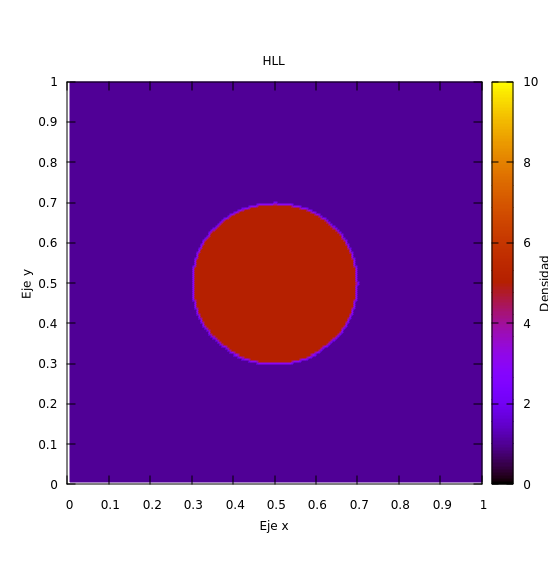
\includegraphics[width=0.5\textwidth]{./Figuras/Pruebas/Prueba_onda_choque/onda_choque3_t_0}
%\caption{Onda de choque en el tiempo $t = 0$, los valores con los que fue suministrado nuestra onda de choque son los mismos que habiamos dicho en el Cuadro \ref{Tabla_parametros} } \label{fig:onda_choque3_t_0}
%\end{figure}
%===================IMAGE_HLL_CENTRADO_T=0===============================


Las condiciones iniciales para la onda de choque son las mismas que las que habiamos tenido en la figura \ref{fig:onda_choque_example}, centrada en el punto $(x,y)=(0.5,0.5)$ cm, su radio es de $r = 0.2 \, \mathrm{cm}$ y al igual que en Lax se presentan 2 ondas, una onda contra el medio, la cual tiene una velocidad constante de $\vec{v}  = 2 \, \mathrm{cm}/\mathrm{s}$ y una onda contra el centro, el radio de la onda se expande a $r = 0.3$ cm al tiempo $t=0.05$ s, mientras que al tiempo $t = 0.1$ s, su radio aumenta hasta $r = 0.38$ cm y disminuye la velocidad de la onda a más de la mitad $\vec{v}=1.8 \, \mathrm{cm}/\mathrm{s}$, entre estas 2 ondas se va creando un vacio (vea figura \ref{fig:HLL-prueba1}).

%===================IMAGE_HLL_CENTRADO_EVOLUCION===============================
\begin{figure}[H]
\centering
\subfigure[$t = 0.05$ s]{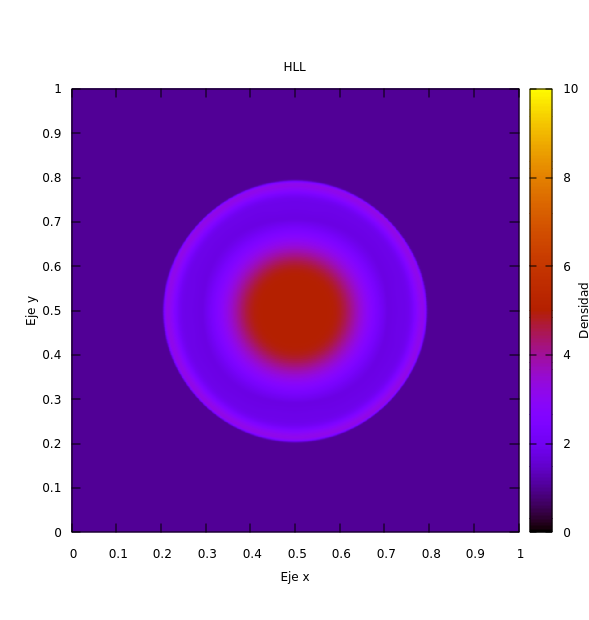
\includegraphics[scale = 0.55]{./Figuras/Pruebas/Prueba_onda_choque/HLL/HLL-sedov_05.png}}
\subfigure[$t = 0.1$ s]{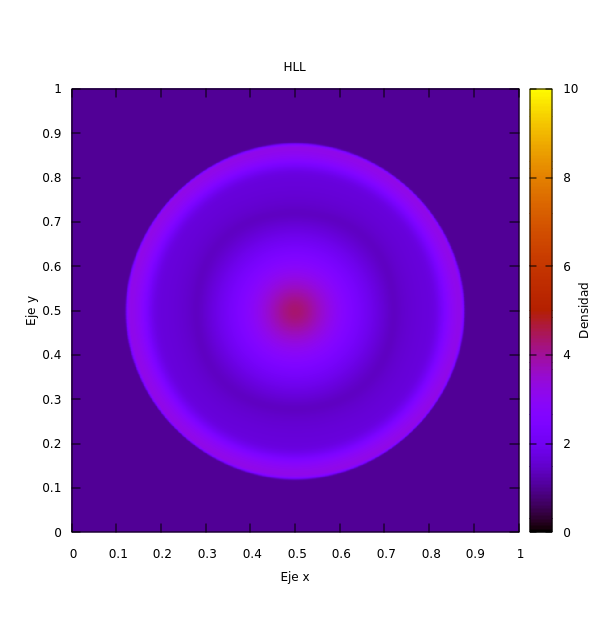
\includegraphics[scale = 0.55]{./Figuras/Pruebas/Prueba_onda_choque/HLL/HLL-sedov_10.png}}
\caption{Evolución de la onda de choque mostrada en la figura \ref{fig:onda_choque_example} usando el método de HLL newtoniano. En el panel a) se muestra la onda de choque a t=0.05s, mientras que en el panel b) se muestra para t=0.10s.} \label{fig:HLL-prueba1}
\end{figure}
%===================IMAGE_HLL_CENTRADO_EVOLUCION===============================


Al igual que lo que paso con Lax, el método HLL muestra el mismo comportamiento. Se pueden ver 2 ondas distintas, una que avanza hacia adelante (\emph{forward shock}) y otra que avanza en sentido contrario, es decir, se contrae y choca con la misma onda (\emph{reverse shock}), la cavidad que se va formando entre estas 2 ondas es prueba de la viscosidad que tiene nuestro método.

%===================IMAGE_HLL_CENTRADO_EVOLUCION_ANALISIS===============================
\begin{figure}[H]
\centering
\subfigure[$t = 0.05$ s]{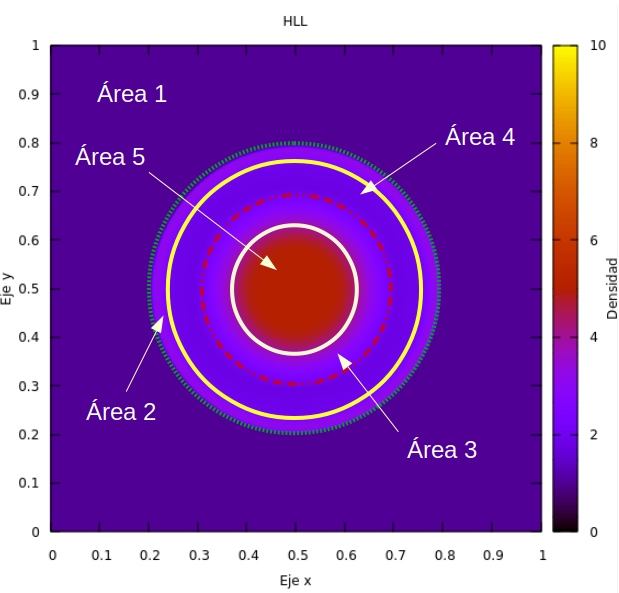
\includegraphics[scale = 0.38]{./Figuras/Pruebas/Prueba_onda_choque/HLL/HLL-sedov_05-analisis.png}}
\subfigure[$t = 0.1$ s]{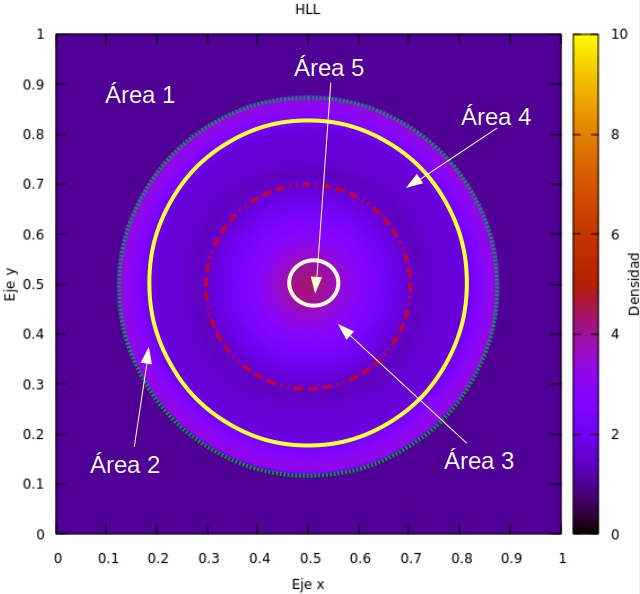
\includegraphics[scale = 0.37]{./Figuras/Pruebas/Prueba_onda_choque/HLL/HLL-sedov_10-analisis.png}}
\caption{\label{fig:HLL-prueba1-analisis}En la onda se logran distinguir 2 ondas distintas al evolucionar la misma. Una onda hacia adelante (\emph{forward shock}) y otra onda que se contrae (\emph{reverse shock}), la separación entre las 2 ondas dejan ver un hueco en la onda de menor densidad. La discusión de las áreas de las ondas es la misma que ya habiamos dicho en figura \ref{fig:Lax-newtoniano-prueba1-analisis} y \ref{fig:Lax-prueba2_no_centrado-analisis}. Se puede ver también como, con el paso del tiempo, las áreas donde barren las ondas incrementan su tamaño.} 
\end{figure}
%===================IMAGE_HLL_CENTRADO_EVOLUCION_ANALISIS===============================


En la siguiente prueba se movió el centro de la onda de choque (ver figura \ref{fig:onda_choque4_t_0}) y este se colocó en el punto $(x,y) = (0.25,0.25)$ [cm], las fronteras funcionaron apropiadamente, el radio de la expansión de la onda al tiempo $t=0.05$ s es de $r = 0.30$ cm y su velocidad a ese instante es de $v = 2.0 \, \mathrm{cm}/\mathrm{s}$. En el tiempo $t = 0.1$  el radio de la onda se expandió a $r = 0.38$ cm, su velocidad de $v = 1.6 \, \mathrm{cm}/\mathrm{s}$

%===================IMAGE_HLL_NO_CENTRADO_T=0===============================
\begin{figure}[H]
\centering
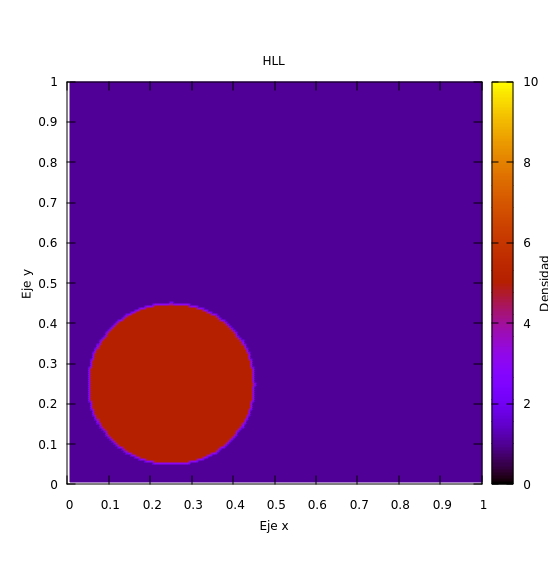
\includegraphics[width=0.5\textwidth]{./Figuras/Pruebas/Prueba_onda_choque/onda_choque4_t_0}
\caption{\label{fig:onda_choque4_t_0}Onda de choque en el tiempo $t = 0$, los valores con los que fue suministrado nuestra onda de choque son los mismos que habiamos dicho en el Cuadro \ref{Tabla_parametros} } \label{fig:onda_choque4_t_0}
\end{figure}
%===================IMAGE_HLL_NO_CENTRADO_T=0===============================

Al pasar el dominio, la onda se sigue comportando como si estuviera centrada, ya que tiene los mismos radios y velocidades de la misma y al llegar al final de nuestro dominio, se nota que no hay ninguna irregularidad de nuestras fronteras (ver figura \ref{fig:HLL-prueba2}).


%===================IMAGE_HLL_NO_CENTRADO_EVOLUCION===============================
\begin{figure}[H]
\centering
\subfigure[$t = 0.05$ s]{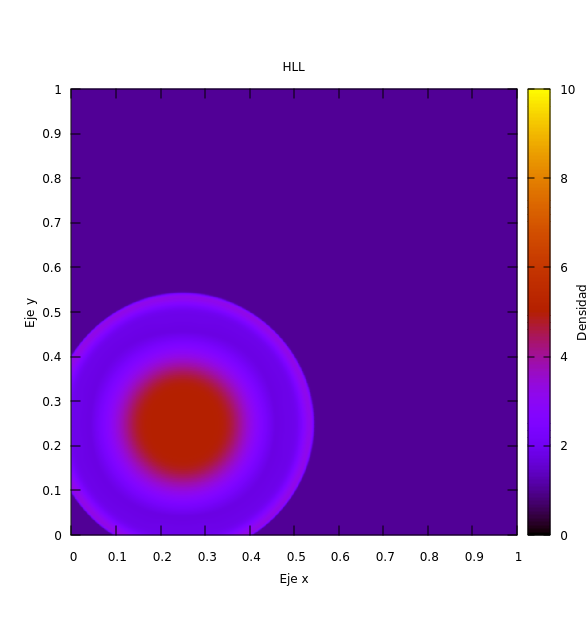
\includegraphics[scale = 0.55]{./Figuras/Pruebas/Prueba_onda_choque/HLL/HLL-sedov2_05.png}}
\subfigure[$t = 0.1$ s]{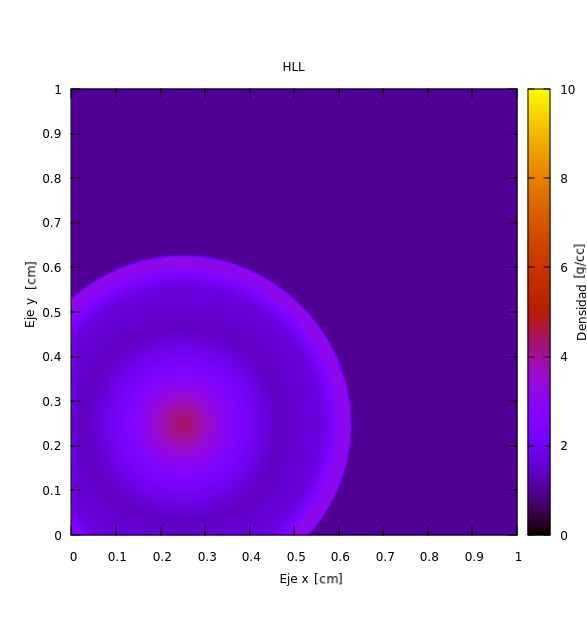
\includegraphics[scale = 0.55]{./Figuras/Pruebas/Prueba_onda_choque/HLL/HLL-sedov2_10.png}}
\caption{\label{fig:HLL-prueba2}Evolución de la onda de choque mostrada en la figura \ref{fig:onda_choque4_t_0} usando el método de HLL newtoniano. En el panel a) se muestra la onda de choque a t=0.05s, mientras que en el panel b) se muestra para t=0.10s.}  
\end{figure}
%===================IMAGE_HLL_NO_CENTRADO_EVOLUCION===============================

Al expandirse la onda, al igual que Lax se separan en 2 ondas. La \emph{forward shock} que va contra el medio a la que hemos llamado el área 1 (veáse figura \ref{fig:HLL-prueba2-analisis}). El área 2, es el material del área 1 que va barriendo la \emph{forward shock}. El área 3 es lo contrario, es decir, es el material barrido del área 5 por la \emph{reverse shock} y entre estas 2 ondas se va formando un hueco entre estas 2 ondas que es el área 4 muestra la viscosidad de nuestro método. Dado  que no se muestran anomálias en la evolución de nuestra onda cerca de las fronteras y que estas tienen las velocidades y radios a los instantes de tiempo especificados, podemos decir que nuestro código funciona bien.
%===================IMAGE_HLL_NO_CENTRADO_EVOLUCION_ANALISIS===============================
\begin{figure}[H]
\centering
\subfigure[$t = 0.05$ s]{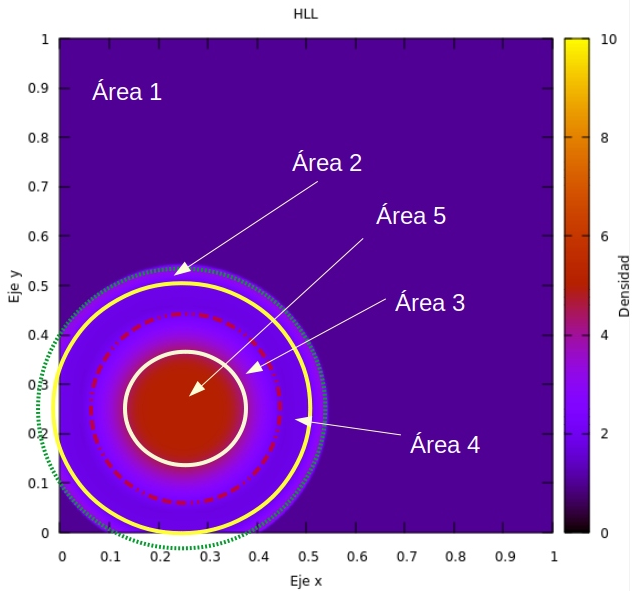
\includegraphics[scale = 0.55]{./Figuras/Pruebas/Prueba_onda_choque/HLL/HLL-sedov2_05-analisis.png}}
\subfigure[$t = 0.1$ s]{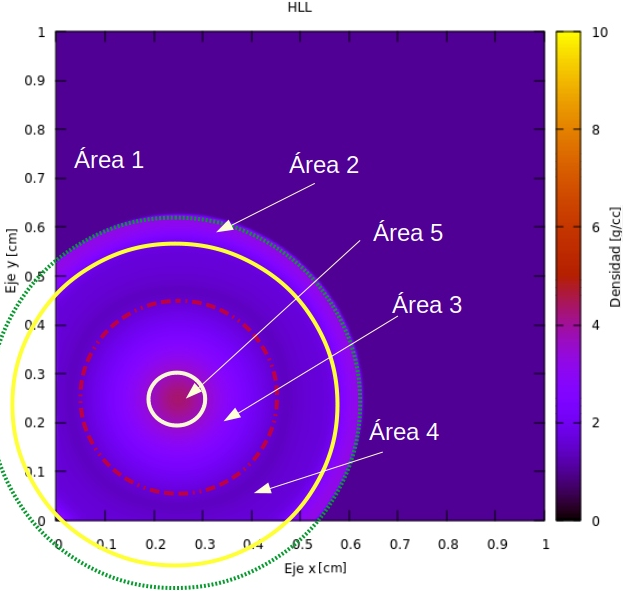
\includegraphics[scale = 0.54]{./Figuras/Pruebas/Prueba_onda_choque/HLL/HLL-sedov2_10-analisis.png}}
\caption{\label{fig:HLL-prueba2-analisis}Las áreas mostradas en el panel a) y en el panel b) son las mismas discutidas en la figura \ref{fig:HLL-prueba1-analisis}.}
\end{figure}
%===================IMAGE_HLL_NO_CENTRADO_EVOLUCION_ANALISIS===============================





En esta sección, vamos a comparar las diferencias que hay entre el método de Lax y el HLL. Las ondas que vamos a ocupar son las de las figuras \ref{fig:Lax-newtoniano_sedov-3-5} y la \ref{fig:HLL-prueba1}. La onda esta centrada en el punto $(x,y)=(0.5,0.5)$

%\begin{figure}[H]
%\centering
%\subfigure[]{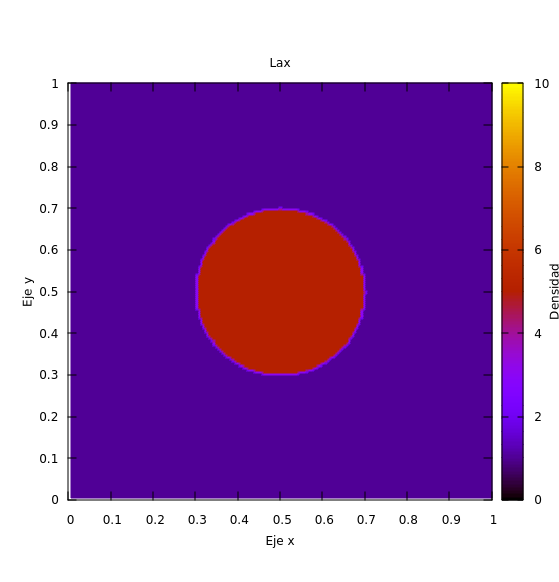
\includegraphics[width=0.45 \textwidth]{./Figuras/Pruebas/Prueba_onda_choque/onda_choque1_t_0}}
%\subfigure[]{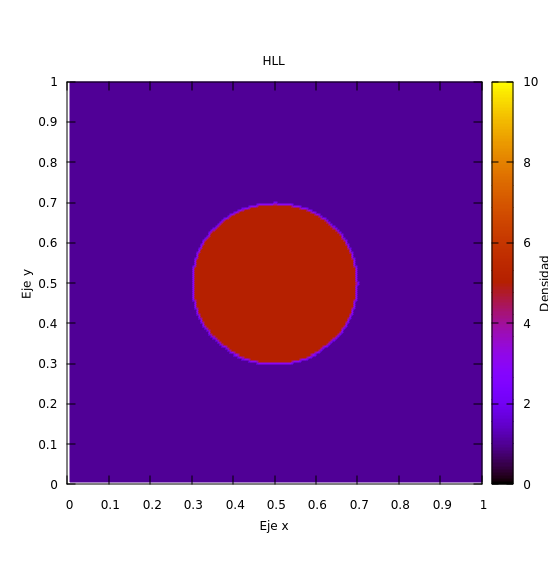
\includegraphics[width=0.465 \textwidth]{./Figuras/Pruebas/Prueba_onda_choque/onda_choque3_t_0}}
%\caption{Condición inicial ($t = 0$) misma para las 2 ondas de choque usando los dos métodos que hemos utilizado que es el de Lax y el de HLL (con $\rho_{in}=5.0, \, v_{x_{in}}=v_{y_{in}}=0.0, \, P_{in}=10.0$ y $E_{in}=3.75$), de radio interno $R_{in} = 0.2$ cm. que se va a expandir sobre un medio (con $\rho_{out}=1.0$  y $ P_{out}=0.1$) estático. Véase el Cuadro \ref{Tabla_parametros} para más detalles.} \label{fig:comparacion_inicial_lax_hll_NR}
%\end{figure}


La onda de Lax al tiempo  $t = 0.05$ s (ver figura \ref{fig:Lax-newtoniano_sedov-3-5}) tiene un radio $r=0.31$ cm y una velocidad $v = 2.2 \, \mathrm{cm}/\mathrm{s}$, mientras que la onda de HLL (ver figura \ref{fig:HLL-prueba1}) tiene un radio $r = 0.31$ y una velocidad $v = 2.2 \, \mathrm{cm}/\mathrm{s}$. Al avanzar la onda se ve una diferencia entre el método de Lax y HLL, la onda contra el centro de la onda se ve más difusa en HLL que con Lax, por lo que se puede concluir que HLL es menos viscoso y resuelve mejor las discontinuidades.


\begin{figure}[H]
\centering
\subfigure[]{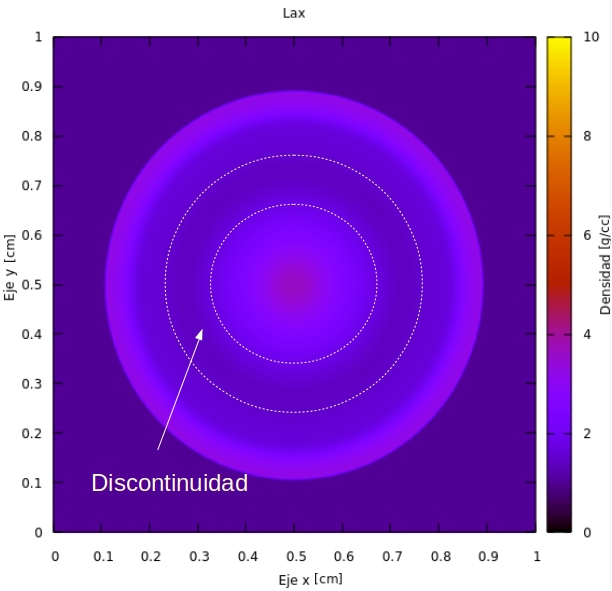
\includegraphics[scale = 0.50]{./Figuras/Pruebas/Prueba_onda_choque/Lax-HLL-new/comparacion1}}
\subfigure[]{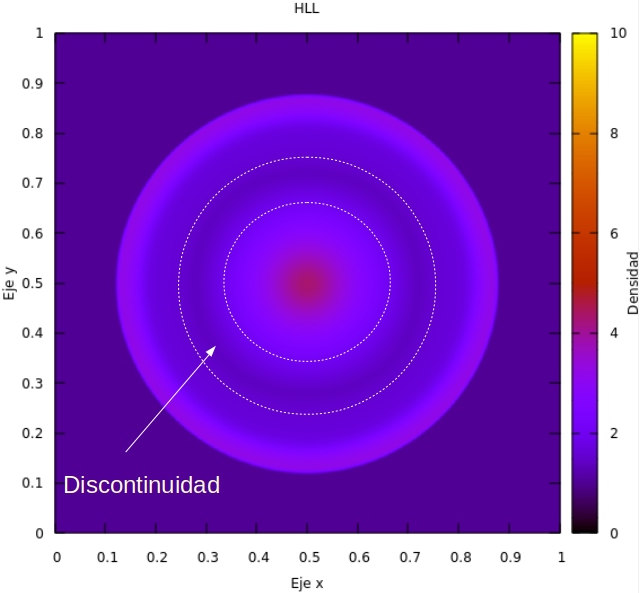
\includegraphics[scale = 0.50]{./Figuras/Pruebas/Prueba_onda_choque/Lax-HLL-new/comparacion2}}
\caption{\label{fig:Lax-hll-newtoniano1}Las ondas de choque están establecidas al tiempo $t = 0.5$, ambas imágenes tienen una resolución de 500x500, mientras que Lax (panel a)) es un poco más rápido que HLL (panel b)), HLL tiene menor viscosidad en la zona de discontinuidad.}  
\end{figure}

\begin{figure}[H]
\centering
\includegraphics[width=1.0\textwidth]{./Figuras/Pruebas/expansion_radial/expansion_radial_newtoniano}
\caption{\label{fig:expansion_radial_newtoniano}Expansión del radio de la onda de choque conforme avanza el tiempo. La recta verde muestra el crecimientro del radio usando el método de Lax, mientras que la recta roja es usando HLL. } 
\end{figure}


La zona de discontinuidad es donde tanto la \emph{forward shock} y la \emph{reverse shock} se separan. En las 2 imágenes, aunque es mínima, se puede notar una difuminación mayor en Lax en esta zona. Por esto podemos decir que HLL es un método para resolver este tipo de discontinuidades. Al dispersarse por completo el centro de la onda, para ambas, se puede ver con mejor claridad que hay 2 diferentes tipos de onda, una contra el medio y otra contra en centro de la misma, para Lax, el radio toma el valor $r = 0.38$ y una velocidad $v = 1.8 \, \mathrm{cm}/\mathrm{s} $. En el caso de HLL es el mismo radio $r = 0.38 $ cm y la misma velocidad $v = 1.8 \, \mathrm{cm}/\mathrm{s}$.

\begin{figure}[H]
\centering
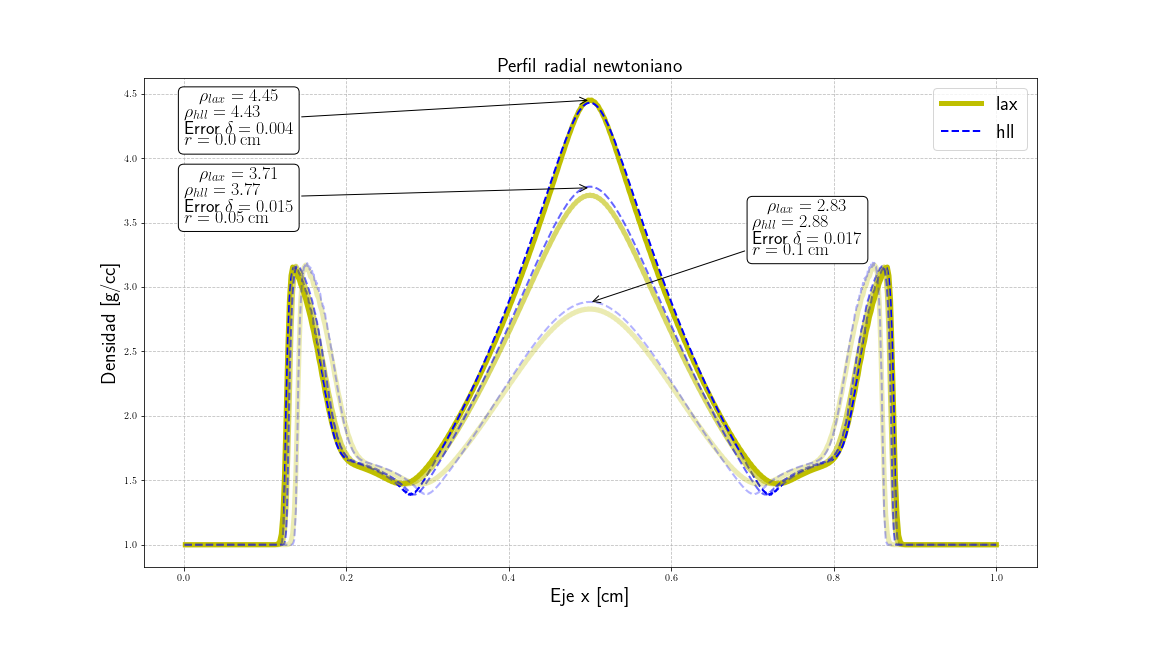
\includegraphics[scale = 0.4]{./Figuras/Pruebas/perfil_radial/perfil_radial_t_10}
\caption{Perfil radial de la onda de choque al tiempo $t = 0.1$ s, la linea verde corresponde al método de Lax, mientras que la linea roja punteada corresponde al método de hll.}
\end{figure}


\subsection{Caso relativista} 
 %200X200

\subsubsection{Lax}
Para el caso relativista, usaremos otros valores en nuestra onda de choque, debido a que queremos que la velocidad con la que se expande nuestra onda tenga velocidades cercanas a la de la luz.

\begin{table}[htbp]\label{Tabla_parametros_relatividad}
\begin{center}
\begin{tabular}{|c|c|c|}
\hline 
\textbf{Parámetro} & \textbf{Descripción} & \textbf{valor} \\ 
\hline 
$R_{in}$ & Radio interno de la onda expansiva & $0.2\times10^{10}$ \\ 
\hline 
$\rho_{in}$ &  Densidad interna de la onda expansiva & $10^{-3}$ \\ 
\hline 
$\rho_{out}$ &  Densidad del medio  & $10^{-10}$ \\
\hline 
$P_{int}$ & Presión interna de la onda expansiva & $2\times10^{18}$ \\ 
\hline 
$P_{out}$ &  Presión del medio  & $\rho_{in} \times 10^{-10}$ \\ 
\hline 
$v_{x_{int}}$ & Velocidad interna en el eje x de la onda expansiva & 0.0 \\ 
\hline 
$v_{y_{int}}$ & Velocidad interna en el eje y de la onda expansiva & 0.0 \\ 
\hline 
$v_{x_{out}}$ & Velocidad en el eje x del medio & 0.0 \\
\hline 
$v_{y_{out}}$ & Velocidad en el eje y del medio & 0.0 \\ 
\hline 
Co & Número de Courant & 0.7 \\ 
\hline 
\end{tabular}
\caption{Parámetros que se utilizarán en las siguientes pruebas que se van a realizar para la onda de choque, estos valores son para fluidos relativistas.}
\end{center}
\end{table}




La onda de choque, aunque tendrá distintos valores que el newtoniano, tendrá un comportamiento parecido a la onda de choque. Las dimensiones del dominio se modificaron para poder evaluar mejor la expansión de la onda. Los valores de nuestras coordenadas x,y tienen valores entre $0$ y $2 \times 10^{10}$ [cm].La presión interna de la onda incrementa 18 ordenes de magnitud y la densidad disminuye a tres ordenes de magnitud, para ver más detalles vea el cuadro \ref{Tabla_parametros_relatividad}. La expansión de la onda disminuye muy rapidamente, su radio inicial es de  $r = 0.2 \times 10^{10}$ cm y estaba centrada en los puntos $(x,y) = (10^{10}, 10^{10})$ cm, ver figura \ref{fig:Lax-relativista}. El radio al tiempo $t=0.025$ s es de $r =  0.24 \times 10^{10}$ y su velocidad $v = 1.0 \times 10^{10} \, \mathrm{cm}/\mathrm{s}$. La velocidad de la onda alcanza casi el 33\% de la velocidad de la luz.

\begin{figure}[H]
\centering
\subfigure[]{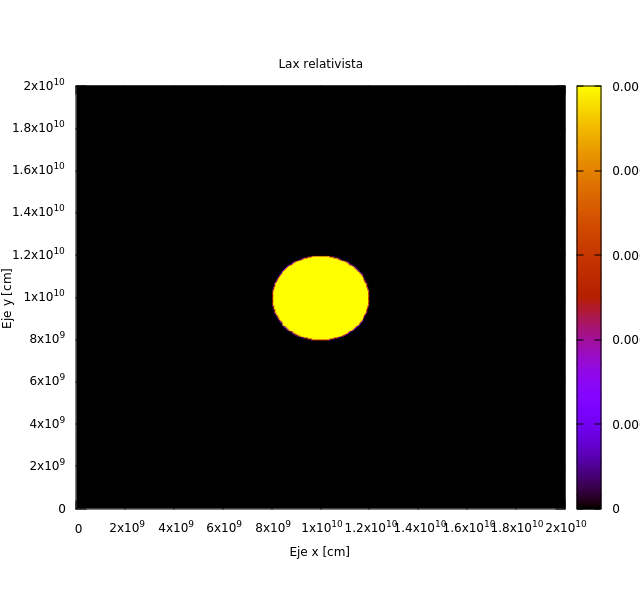
\includegraphics[width=0.45\textwidth]{./Figuras/Pruebas/Prueba_onda_choque/Lax-HLL-rel/bwlax-rel0}}
\subfigure[]{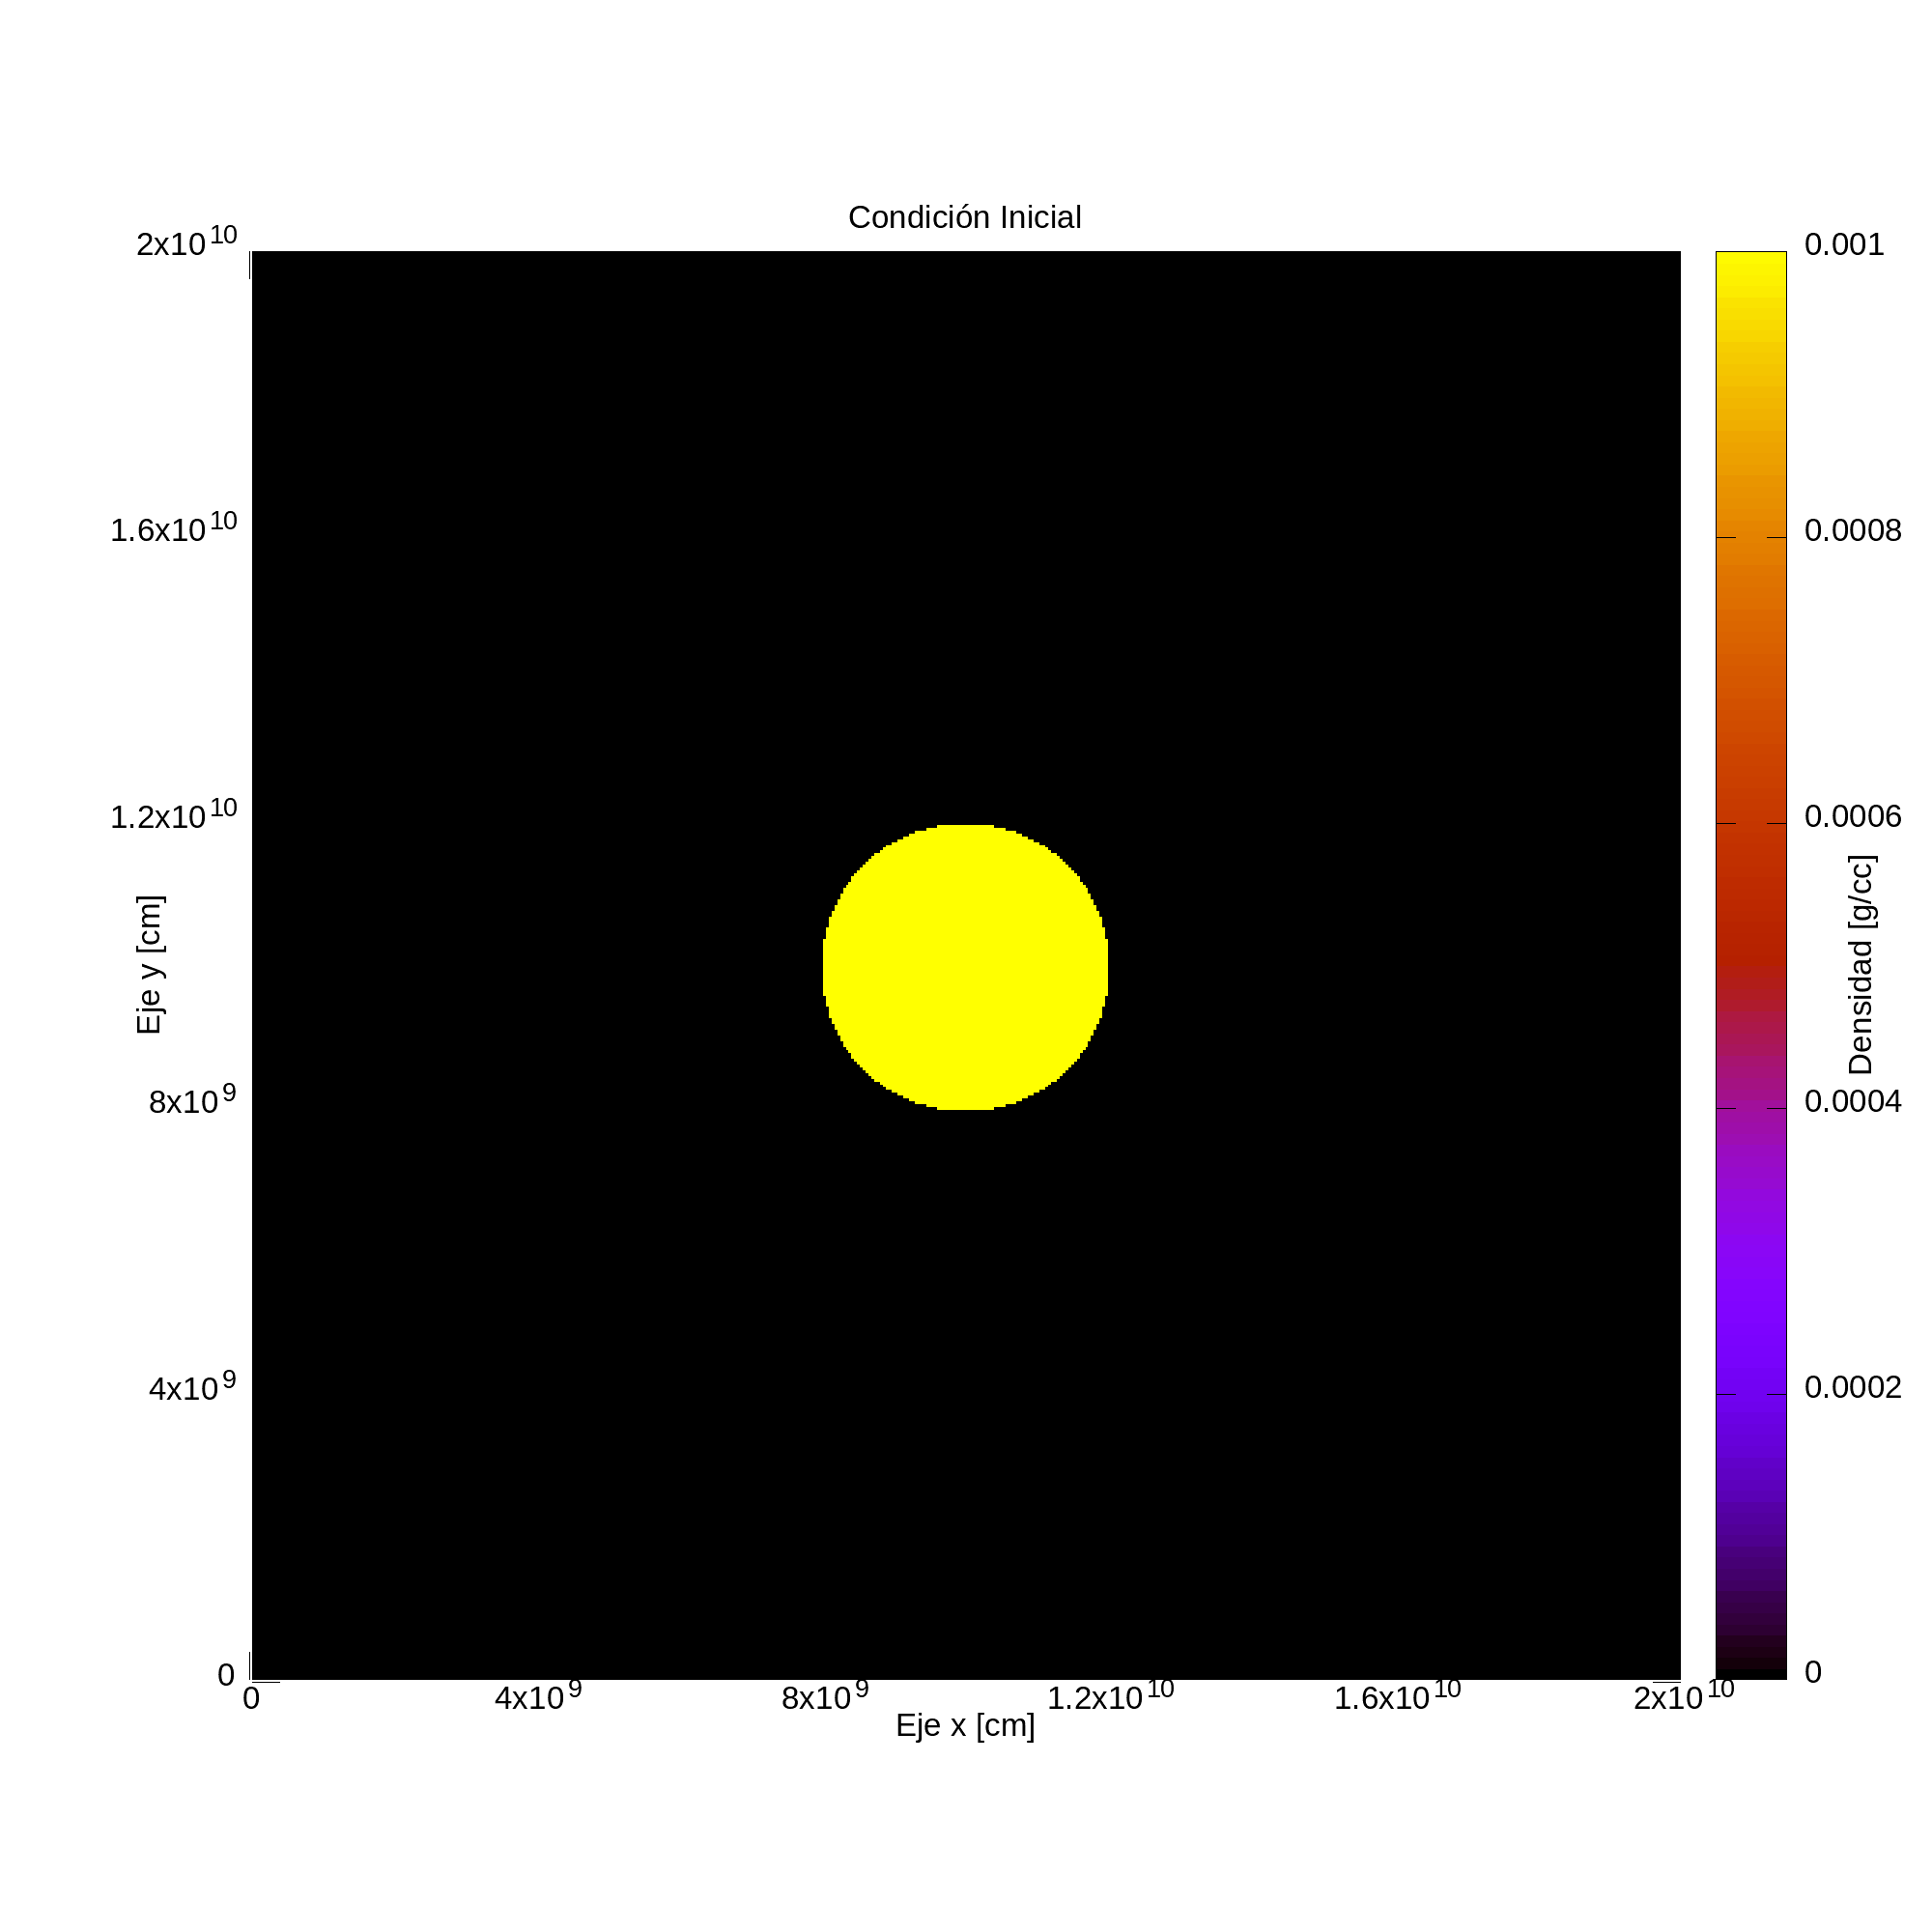
\includegraphics[scale = 0.45]{./Figuras/Pruebas/Prueba_onda_choque/Lax-HLL-rel/bwlax-rel01}}
\caption{Evaluación de nuestra onda relativista. En el panel a) es al instante $t=0$ s y en el panel b) es al tiempo $t = 0.05$ s. La velocidad que alcanza la onda en los primeros instantes de su vida es de $v = 1.0 \times 10^{10} \, \mathrm{cm}/\mathrm{s}$, casi un 33\% de la velocidad de la luz} \label{fig:Lax-relativista}
\end{figure}

Para revisar si nuestra onda, usando el método de Lax, no tiene problemas en la frontera por usar velocidades muy altas; se movió el centro de la misma al punto $(x,y) = (0.3 \times 10^{10}, 0.3 \times 10^{10})$ cm.

\begin{figure}[H]
\centering
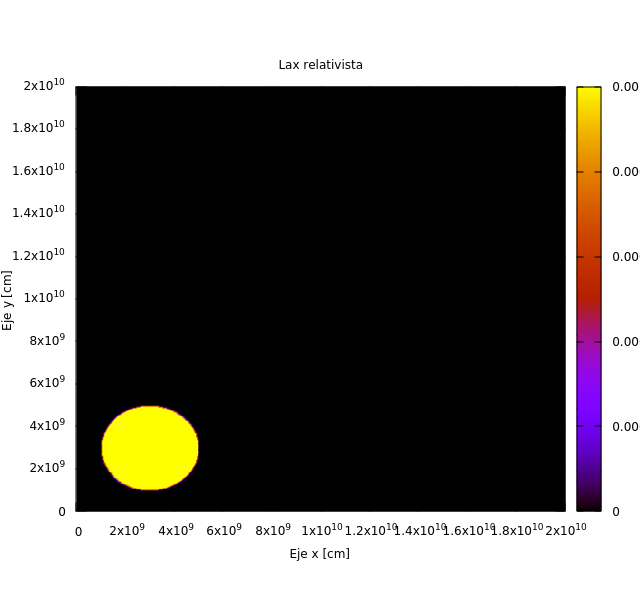
\includegraphics[scale=0.5]{./Figuras/Pruebas/Prueba_onda_choque/Lax-HLL-rel/bwlax-rel0-no-centrado}
\caption{Condición inicial de nuestra onda de choque centredo en el punto $(x,y) = (0.3 \times 10^{10}, 0.3 \times 10^{10})$ cm. La densidad $\rho$, presión $P$ y densidad de Energía $E$ son los mismos que desarrollamos para el centrado, vea el cuadro \ref{Tabla_parametros_relatividad}.} \label{fig:bwlax-rel-no-centrado}
\end{figure}

Cuando nuestra onda toca las fronteras, esta evoluciona con normalidad, ya que no se observa alguna anomalía cuando las traspasa. Recordemos que aún seguimos usando la condición de \emph{Outflow}.

La expansión del radio de nuestra onda de choque es lo mismo para el centrado y el no centrado ya que sus radios son $r \approx 10^{9}$ cm.

\begin{figure}[H] 
\centering
\subfigure[]{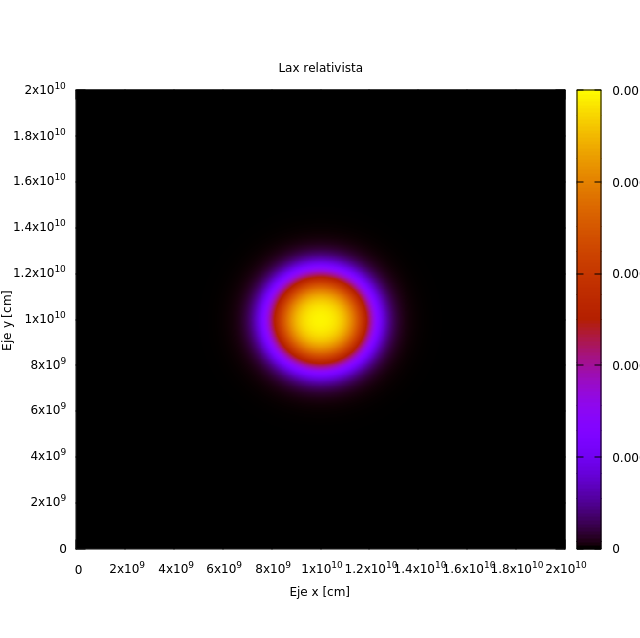
\includegraphics[scale = 0.45]{./Figuras/Pruebas/Prueba_onda_choque/Lax-HLL-rel/bwlax-rel79}}
\subfigure[]{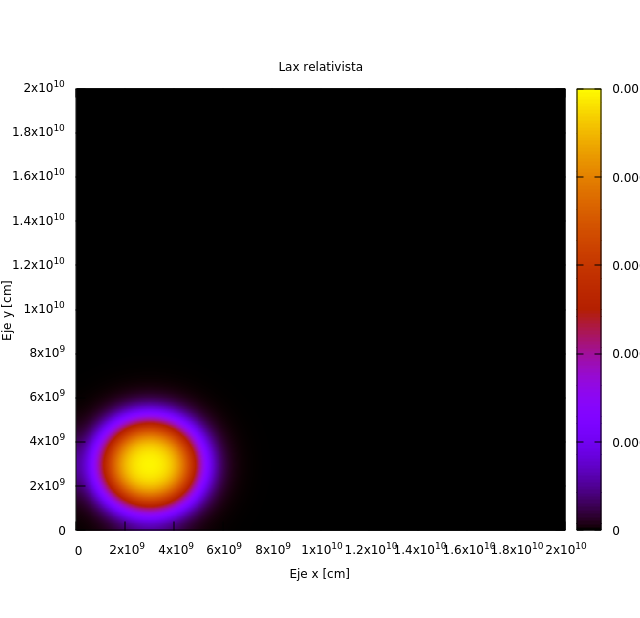
\includegraphics[scale = 0.46]{./Figuras/Pruebas/Prueba_onda_choque/Lax-HLL-rel/bwlax-rel79-no-centrado}}
\caption{Evolución de la onda al tiempo $t = 1.97$ s. En el panel a) se desarrolla la onda de choque centrada (ver figura \ref{fig:Lax-relativista}). En el panel b) se muestra el desarrollo de la onda no centrada (ver figura \ref{fig:bwlax-rel-no-centrado}).} \label{fig:Lax-relativista-t-1.97}
\end{figure}



\subsubsection{HLL}


Se hicieron las mismas pruebas usando el método de HLL. El radio inicial de nuestra onda es el mismo que el que se usó con Lax $r = 0.2 \times 10^{10}$ cm y se desplazó al tiempo $t=0.025$ s $r =  0.24 \times 10^{10}$ con lo que su velocidad fue $v = 1.0 \times 10^{10} \, \mathrm{cm}/\mathrm{s}$. 

\begin{figure}[H] 	
\centering
\subfigure[]{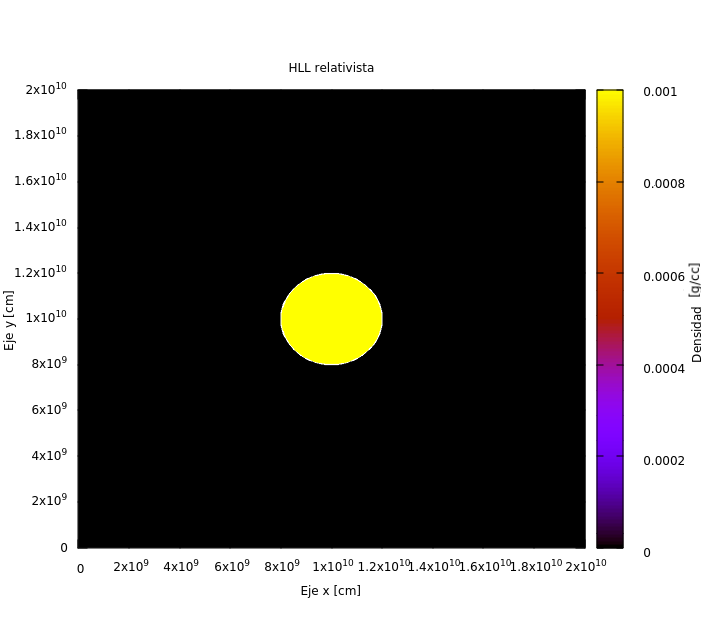
\includegraphics[width=0.5\textwidth]{./Figuras/Pruebas/Prueba_onda_choque/Lax-HLL-rel/bwhll-rel0}}
\subfigure[$t = 0.06$ s]{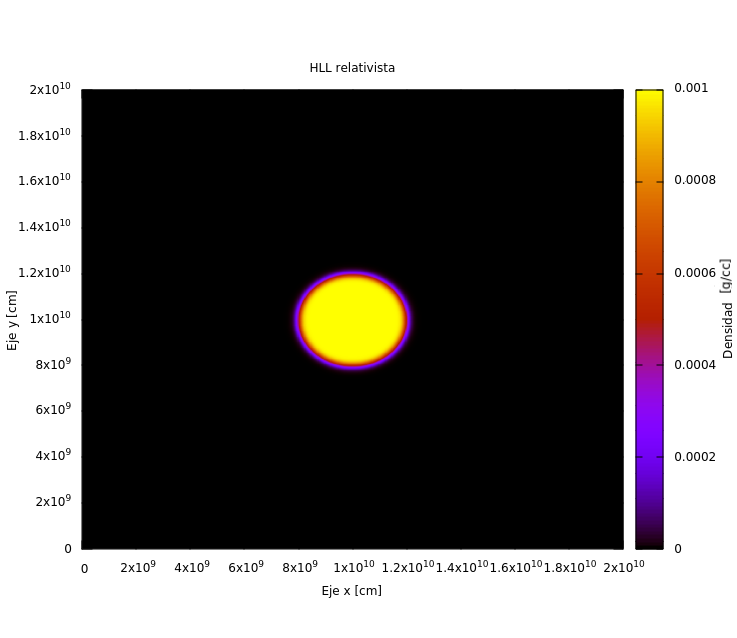
\includegraphics[scale = 0.5]{./Figuras/Pruebas/Prueba_onda_choque/Lax-HLL-rel/bwhll-rel01}}
\caption{Expansión de la onda de choque. En el panel a) se muestra la condición inicial de la onda de choque. En el panel b) se muestra al instante $t = 0.025$ s. La velocidad de la onda decrece rapidamente.} \label{fig:bwhll-rel-centrado}
\end{figure}

Al igual que el método de Lax, la velocidad que alcanza es cerca del 33 \% de la velocidad de la luz.

Se movió el centro de la onda, para revisar que, al igual que el método de Lax, el método de HLL no tuviera problemas con las fronteras.

\begin{figure}[H]
\centering
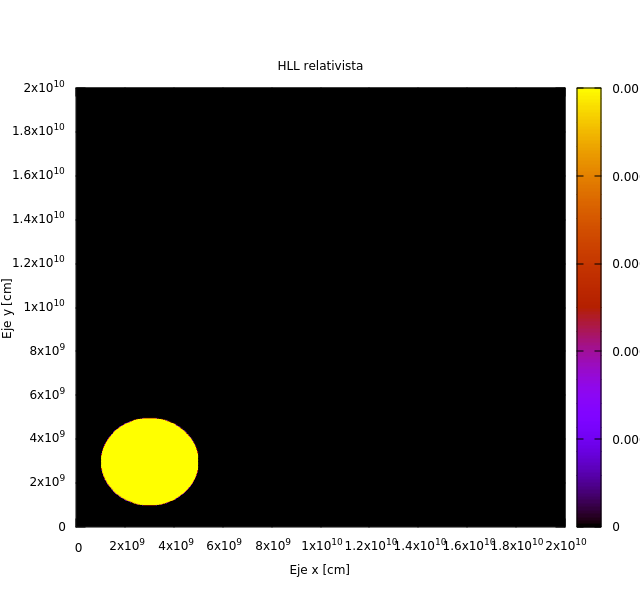
\includegraphics[scale=0.5]{./Figuras/Pruebas/Prueba_onda_choque/Lax-HLL-rel/bwhll-rel0-no-centrado}
\caption{Condición inicial de nuestra onda de choque, usando el método de HLL, centrado en el punto $(x,y) = (0.3 \times 10^{10}, 0.3 \times 10^{10})$ cm. La densidad $\rho$, presión $P$ y densidad de Energía $E$ son los mismos que desarrollamos para el centrado, vea el cuadro \ref{Tabla_parametros_relatividad}.} \label{fig:bwhll-rel-no-centrado}
\end{figure}

El desarrollo al tiempo $t = 1.97$ s, las 2 ondas tanto la centrada como la que no esta centrada tienen el mismo incremento de radio $r \approx 10^{9}$ cm.

\begin{figure}[H]
\centering
\subfigure[]{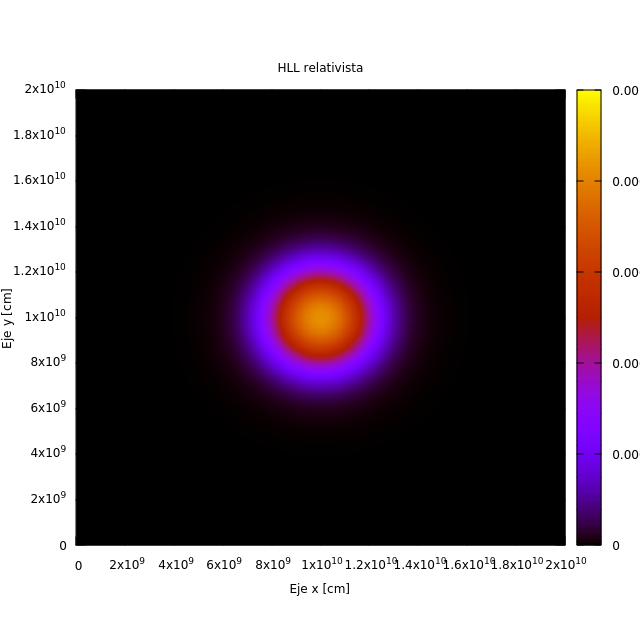
\includegraphics[scale=0.45]{./Figuras/Pruebas/Prueba_onda_choque/Lax-HLL-rel/bwhll-rel79}}
\subfigure[]{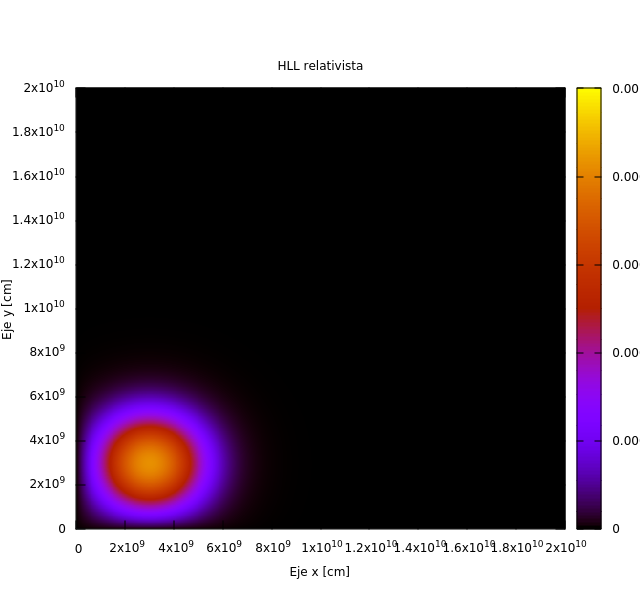
\includegraphics[scale=0.45]{./Figuras/Pruebas/Prueba_onda_choque/Lax-HLL-rel/bwhll-rel79-no-centrado}}
\caption{Evolución de la onda al tiempo $t = 1.97$. En el panel a) se muestra el desarrollo de la figura \ref{fig:bwhll-rel-centrado}. En el panel b) se muestra el desarrollo de la figura \ref{fig:bwhll-rel-no-centrado}, asi como un correcto funcionamiento de onda sobre las fronteras.}
\end{figure}




\subsubsection{Lax vs HLL}
En la última parte de la onda de choque vamos a comparar los dos métodos que hemos visto hasta ahora.


\begin{figure}[H] \label{fig:analisis_onda_relativista_lax1}
\centering
{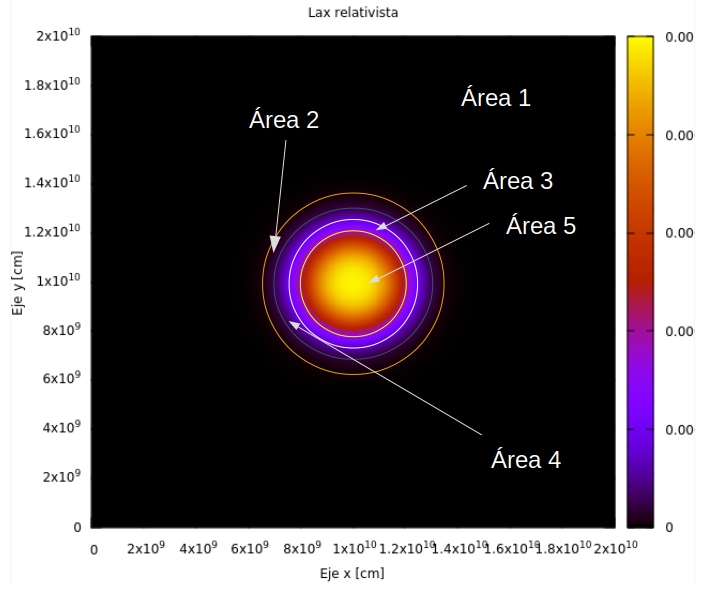
\includegraphics[scale=0.5]{./Figuras/Pruebas/Prueba_onda_choque/Lax-HLL-rel/bwlax-rel79-analisis}}
\caption{Análisis de la onda de choque al tiempo $t = 1.97$ s. Se pueden apreciar las mismas áreas que vimos en el caso newtoniano. La discontinuidad que hay en el área 4 no se puede notar como en el caso no relativista.}
\end{figure}

A pesar de las dificultades, podemos ver las mismas áreas que en el caso newtoniano. Donde el área 1 es el medio que no ha sido tocado, el área 2 el material barrido por la \emph{forward shock}, que podemos notar que su densidad es casi la misma que el medio ambiente. El área 3 es el material que ha sido tocado por la \emph{reverse shock}. El área 4 muestra la discontinuidad que se genera entre estas 2 ondas y el área 5 el material que no ha sido tocado por la \emph{reverse shock}.

\begin{figure}[H] \label{fig:analisis_onda_relativista_hll1}
\centering
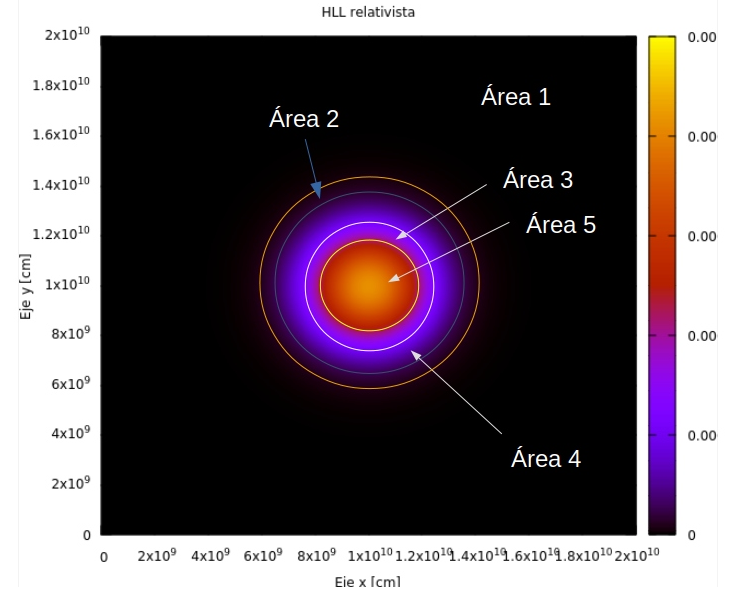
\includegraphics[scale=0.5]{./Figuras/Pruebas/Prueba_onda_choque/Lax-HLL-rel/bwhll-rel79-analisis}
\caption{Las áreas apreciadas son muy parecidos al método de Lax}
\end{figure}

Se visualizó un perfil radial de las figuras \ref{fig:analisis_onda_relativista_lax1} y \ref{fig:analisis_onda_relativista_hll1} y se sobrepusieron en la figura \ref{fig:perfil_radial_relativista_newtoniano}, el error que hay entre ellas al comparar los picos de las densidades mas altas es apenas del $\approx 4 \, \%$

\begin{figure}[H] \label{fig:perfil_radial_relativista_newtoniano}
\centering
\subfigure[]{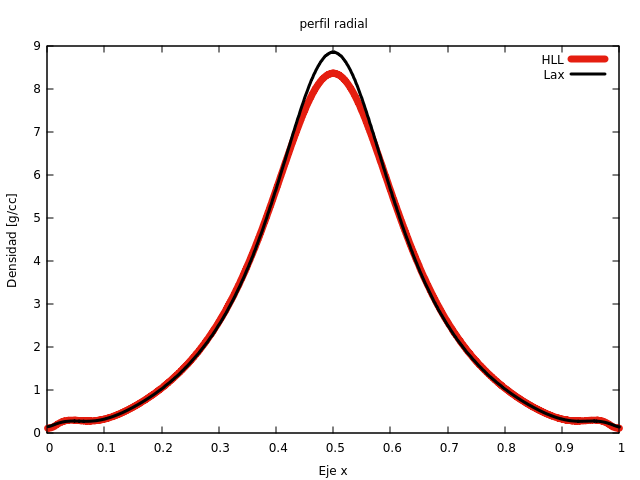
\includegraphics[scale = 0.50]{./Figuras/Pruebas/perfil_radial/relativistico_densidad.png}}
\caption{La diferencia que hay entre los picos de densidad, sugieren un error aproximado del $\approx 4 \, \%$}
\end{figure}


\section{Jet}

El jet  es una emisión delgada de gas a velocidades altas, que se propaga en un medio ambiente gaseoso. Para poder simular nuestro jet vamos a inyectar continuamente energía y presión de un lado de la frontera con velocidades, en nuestro caso, cercanas a la de la luz.

\begin{figure}[H]
\centering
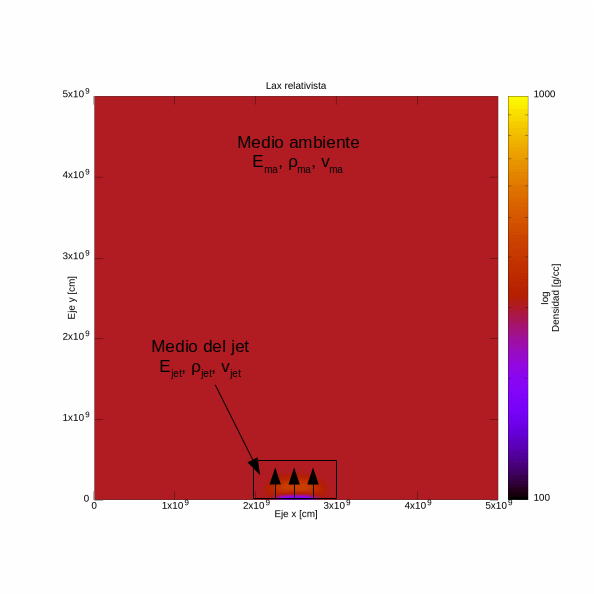
\includegraphics[scale=0.45]{./Figuras/Pruebas/Prueba_jet/jet_ejemplo}
\caption{Para poder simular nuestro jet, se inyectarán energía y presión constante del lado de la parte de abajo de nuestro dominio. Sobre esta parte, sólo se inyectara a una pequeña fracción de este lado en el centro.}
\end{figure}

Las pruebas del jet van a ser en un medio con una densidad más grande que con la que se le está inyectando al jet. En general para todas las pruebas la densidad del jet será de $\rho_{jet}  = 100 \, g/\mathrm{cm}^2$, la presión será $P_{jet} = 20 \times \rho_{jet} \frac{g}{\mathrm{s^2} \mathrm{cm}}$, es decir, la presión sera 20 veces mas grande que la magnitud de la densidad. Para nuestro medio ambiente, la densidad va a variar pero se empezará con un valor de $\rho_{ma}  = 300 \, g/\mathrm{cm}^2$, y al igual que nuestro jet $P_{ma} = 20 \times \rho_{ma} \frac{g}{\mathrm{s^2} \mathrm{cm}}$. La velocidad de los jets tendrán dirección solo en el eje $y$, con una velocidad de $v_{jet_{y}} = 0.9797959 \times c \, \mathrm{cm}/ \mathrm{s}$.

\subsection{Lax}

Las pruebas del jet van a ser usando Lax, van a ser usando una densidad $\rho_{jet}  = 100 \, g/\mathrm{cm}^2$, con una resolución de 500 pixeles. El tamaño de nuestro dominio será cuadrado, con una longitud de $x = y = 1\times 10^9 \, \mathrm{cm}$. Se puede ver como el jet desplaza el material del medio ambiente y va creando un hueco donde hay menor densidad. A esta parte se le conoce como el capullo del jet.

\begin{figure}[H] \label{fig:jet_ma_300}%Snapshot 20 
\centering
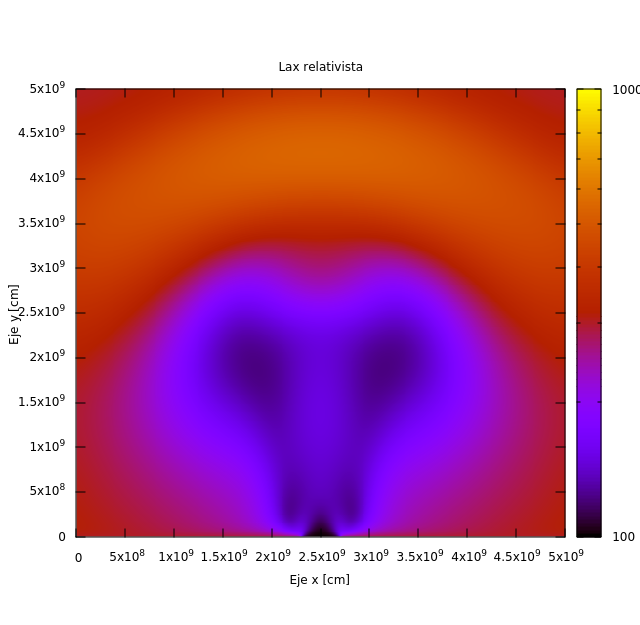
\includegraphics[scale=0.5]{./Figuras/Pruebas/Prueba_jet/lax/jet_100_t_20} 
\caption{Ejección de un jet al tiempo $t = 0.2$ s, con una densidad  $\rho = 100 \, \mathrm{g}/\mathrm{cm}^3$, una velocidad de sobre el eje y $v_y = 0.9797959 \, \mathrm{c}$  y una presión 20 veces la  magnitud de la densidad $P = 20 \times \vert \rho \vert$. La densidad del medio ambiente es $\rho = 300 \, \mathrm{g}/\mathrm{cm}^3$ y la presión es 20 veces mayor la del medio ambiente.}
\end{figure}

La siguiente prueba fue haciendo nuestro medio ambiente más denso, pero las condiciones del jet como presión y velocidad se mantuvieron iguales que en nuestra anterior prueba. El jet mostró mas dificultades al escapar debido a la densidad y presión más elevadas. Se formó al igual que en la figura \ref{fig:jet_ma_300} una menor densidad debido al desplazamiento de materia que hizo el jet.

\begin{figure}[H] \label{fig:jet_100_t_20_ma_500}%Snapshot 20
\centering
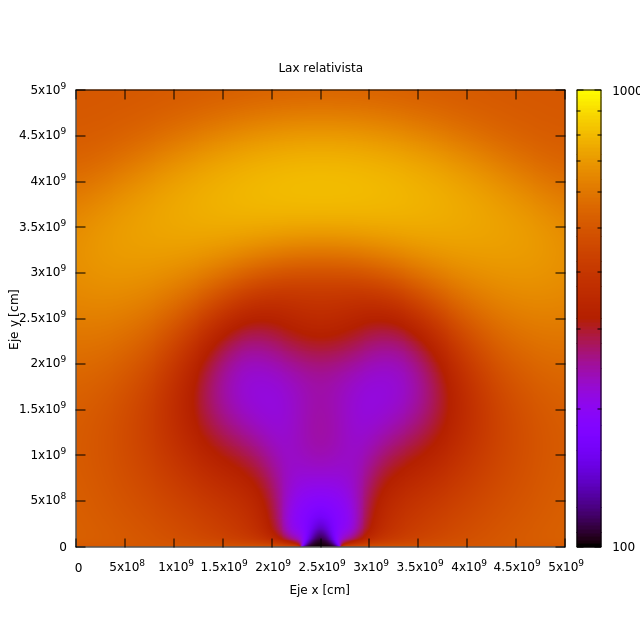
\includegraphics[scale=0.5]{./Figuras/Pruebas/Prueba_jet/lax/jet_100_t_20_ma_500} 
\caption{Se puede apreciar perfectamente como la velocidad del jet es menor con respecto a \ref{fig:jet_ma_300} debido a que la densidad de nuestro medio ambiente es 1.6 veces mas grande.}
\end{figure}

\subsection{HLL}

La siguiente parte fue usando el método de HLL, el cual ha mostrado ser un método más difícil de aplicar debido al tiempo de ejecución que lleva en un ordenador. Al igual que el método de Lax, este se hizo con una resolución de 500x500 pixeles.

\begin{figure}[H] \label{fig:jet_hll_100_ma_300_500pix} %Snapshot 20
\centering
\includegraphics[scale=0.5]{./Figuras/Pruebas/Prueba_jet/hll/jet_hll_100_ma_300_500pix} 
\caption{La imágen de HLL tiene una resolución de 500x500 píxeles. El tiempo es $t =0.2 $ s. El método de HLL nos muestra una distribución de las densidades entre el medio ambiente y el del jet casi homogeneas, dicho de otra manera, sin muchas discontinuidades. }
\end{figure}

Al incrementar la densidad del medio externo a 500 g/cc, usando el método de HLL, se puede ver que la interaccion del jet con el medio ambiente se hace más difícil de apreciar dado que no hay mucha diferencia de densidad entre estas dos interacciones. Ademas de que con este método no podemos apreciar, apesar de la resolución que estamos introduciendo, las discontinuidades presentes entre el jet y el medio ambiente. 

\begin{figure}[H] %Snapshot 20
\centering
\includegraphics[scale=0.5]{./Figuras/Pruebas/Prueba_jet/hll/jet_hll_100_ma_500_500pix} 
\caption{Esta prueba tiene una densidad de medio ambiente es de 500 g/cc. La interacción que hay entre el medio ambiente y el jet es pobremente notoria apesar de la resolución que estamos ejerciendo.}
\end{figure}

\subsection{Comparación Lax-HLL}

Al ver las figuras \ref{fig:jet_ma_300} y \ref{fig:jet_hll_100_ma_300_500pix} podemos notar grandes diferencias entre ambos métodos. En la figura \ref{fig:analisis_jet_densidad_300}, en los ovalos blancos podemos ver que la densidad usando el método de Lax, es sutilmente mas grande que en el que vemos usando HLL. En los par de ovalos negros erguidos se puede ver una menor densidad en Lax pero que no existe en HLL. Además que en el óvalo acostado, donde el jet es inyectado, es donde ocurre la mayor anomalía dado que en HLL no se registra una densidad de 100 g/cc (que es la densidad de nuestro jet).

\begin{figure}[H] \label{fig:analisis_jet_densidad_300} %Snapshot 20
\centering
\includegraphics[scale=0.5]{./Figuras/Pruebas/Prueba_jet/analisis_jet_densidad_300} 
\caption{La diferencia que hay entre HLL (panel izquierdo) y Lax (panel derecho) es notoriamente mayor, dado que HLL en el ovalo blanco muestra una menor densidad que Lax. En los óvalos negros muestra una densidad mayor a diferencia de Lax y la anomalía mas grande es en la parte de abajo donde se inyecta el jet dado que no se muestra una densidad de 100 g/cc como se esta inyectando el jet.}
\end{figure}

En la prueba con densidad de medio ambiente mayor sigue habiendo grandes diferencias entre ambos métodos. Al igual que en la figura \ref{fig:analisis_jet_densidad_300} en el óvalo blanco de la figura \ref{fig:analisis_jet_densidad_500} la densidad sigue siendo mayor en Lax que en HLL y en el círculo negro se nota una densidad mucho menor en Lax, que en HLL.

\begin{figure}[H] \label{fig:analisis_jet_densidad_500} %Snapshot 20
\centering
\includegraphics[scale=0.5]{./Figuras/Pruebas/Prueba_jet/analisis_jet_densidad_500} 
\caption{La comparación entre las 2 figuras aún con una densidad de medio ambiente de $300 \, g/\mathrm{cm}^2 $ sigue siendo significativa dado la diferencia de densidades que fueron marcados con los ovalos blancos y en los círculos negros.}
\end{figure}
\chapter{Medios de densidad}

En este capítulo, probaremos el código con diferentes medios de densidad, con el fin de ver las interacciones que hay entre el jet y su entorno. El método que vamos a usar para realizar nuestras pruebas va a ser el de Lax, dado que, como hemos visto hasta ahora, el tiempo de ejecución del programa ha sido mucho menor usandolo asi como la viscosidad que se ha visto en nuestros gráficos.

\section{SGRB en medio de densidad 1}
En este primer subsección tomaremos una valor de una densidad de medio ambiente muy bajo, es decir, que el jet este expuesto al vacío, la densidad del jet que vamos a utilizar va a ser de $\rho_{jet} = 100 \, g/\mathrm{cm}^3 $ y la presión que vamos a utilizar va a ser de 20 veces mayor que la magnitud de la densidad. La densidad del medio ambiente tendrá un valor de $\rho_{jet} = 10^{-10} \, g/\mathrm{cm}^3 $, al igual que el jet, su presión será 20 veces mas grande el módulo de la densidad. La velocidad del jet disminuye a $v = 0.83c$

\begin{figure}[H]
\centering
\subfigure[]{\includegraphics[scale = 0.450]{./Figuras/densidad_de_medios_ambientes/medio_nulo_10a}}
\subfigure[]{\includegraphics[scale = 0.450]{./Figuras/densidad_de_medios_ambientes/medio_nulo_80a}}
\caption{Al tener únicamente velocidad sobre el eje y, el jet forma perfectamente un cilindro. Pero se puede observar que el jet se expande simétricamente sobre el eje x. Esta expansión sobre el eje x es solo para densidades muy bajas comparadas a la del jet.}
\end{figure}

\section{SGRB en medio de densidad 2}

Ahora aumentaremos la densidad de nuestro medio ambiente, esta será 10 veces más grande que nuestro jet, es decir, tendrá una densidad $\rho_{ma} = 1000 \, g/\mathrm{cm}^3 $. El jet, en sus primeros instantes de vida, desplaza la materia isotrópicamente. Enseguida se puede ver, que a pesar de que el jet esta colimado, forma un pequeño capullo donde la densidad es mas grande que en sus alrededores como se muestra en en panel b) de la figura \ref{fig:medio_ambiente_1000}.

\begin{figure}[H] \label{fig:medio_ambiente_1000}
\centering
\subfigure[]{\includegraphics[scale = 0.450]{./Figuras/densidad_de_medios_ambientes/medio_1000gcc_10a}}
\subfigure[]{\includegraphics[scale = 0.450]{./Figuras/densidad_de_medios_ambientes/medio_1000gcc_70a}}
\caption{En los primeros instantes $t~0.1$ s el jet desplaza la materia del medio ambiente isotrópicamente, al ir avanzando, el jet va desplazando el material y se reduce su velocidad a $v = 0.4c$}
\end{figure}

\section{Comparación con el GRB170817}


\chapter{Conclusiones}



\appendix
\chapter{Código}\label{aped.A}

El programa está escrito en lenguaje FORTRAN se compone de un módulo principal el cual está compuesto de un programa principal y este a su vez llamará a varias subrutinas:
\begin{itemize}
\item \textbf{initconds}: Esta subrutina calculará los valores iniciales que le demos al programa

\item \textbf{output}: Devuelve un archivo con los datos que se calculan con el método de Lax

\item \textbf{Courant}: Calcula el paso temporal

\item \textbf{ulax}: Calcula el paso siguiente de las variables conservadas

\item \textbf{boundaries}: En esta parte puedes definir las fronteras a utilizar como outflow o las condiciones para las del jet

\item \textbf{fluxes}: Calculo de los flujos
\end{itemize}

Al usar las ecuacuaciones hidrodinámica relativistas, se agregan 2 subrutinas más:

\begin{itemize}
\item \textbf{uprim}: Este módulo es agregado para poder desacoplar las variables conservadas

\item \textbf{newraph}: Calcula el método de Newton-Rapson será de gran utilidad en el desacoplamineto de las variables conservadas y así obtener nuestras primitivas
\end{itemize}

\begin{lstlisting}[frame=single] 
do i=0,nx+1
  do j=0,ny+1
   
   x=float(i)*dx 	! obtain the position x_i
   y=float(j)*dy 	! obtain the position y_j
   rad=sqrt((x-xc)**2+(y-yc)**2)
   
   if (rad < 0.1) then
   
     lorin=1/sqrt(1-(vxin**2+vyin**2))
     hin=1.+gamma/(gamma-1.)*pin/rhoin
           
     u(1,i,j)=rhoin*lorin
     u(2,i,j)=rhoin*vxin*lorin**2*hin
     u(3,i,j)=rhoin*vyin*lorin**2*hin
     u(4,i,j)=rhoin*lorin**2*hin-pin
    
    else
    
     lorout=1./sqrt(1.-(vxout**2+vyout**2))
     hout=1.+gamma/(gamma-1.)*pout/rhoout
     
     u(1,i,j)=rhoout*lorout
     u(2,i,j)=rhoout*vxout*lorout**2*hout
     u(3,i,j)=rhoout*vyout*lorout**2*hout
     u(4,i,j)=rhoout*lorout**2*hout-pout
     

\end{lstlisting}
y para los fluidos en la subrutina de fluxes
\begin{lstlisting}[frame=single]
          f(1,i,j)=rho*vx*lor
          f(2,i,j)=rho*vx*vx*lor**2*h+P
          f(3,i,j)=rho*vx*vy*lor**2*h
          f(4,i,j)=rho*vx*lor**2*h

          g(1,i,j)=rho*vy*lor
          g(2,i,j)=rho*vx*vy*lor**2*h
          g(3,i,j)=rho*vy*vy*lor**2*h+P
          g(4,i,j)=rho*vy*lor**2*h
\end{lstlisting}
Como el código es una iteración, solo la primera vez que itere estaremos bien, pero, al siguiente bucle saldrá mal debido a que nuestros resultados nos están arrojando en principio las variables conservadas, y lo que se requiere es obtener las primitivas.

\section{Condición inicial}
En la subrutína \textit{initconds} se calcularán las condiciones iniciales, tomando los valores de los parámetros del módulo de \textit{globals}, que en este caso son: la densidad $(\rho)$, las velocidades tanto en $x$ como en $y$ $(v_x, v_y)$, la presión $(p)$ y $\Gamma$. Con estas constantes dadas se calcularán nuestras variables conservadas.

\begin{lstlisting}[frame=single] 
!==============================================================================
! In this module we set the initial condition
!------------------------------------------------------------------------------
      subroutine initconds(time,tprint,itprint)
      use globals
      implicit none
      real, intent(out) :: time, tprint
      integer, intent (out) :: itprint
      integer ::i,j
      real :: x,y, rad

!------------------------------------------------------------------------------
! For the 2D circular blast:
! u(1,i,j) = rho(i,j)
! u(2,i,j) = vx(i,j)
! u(3,i,j) = vy(i,j)
! u(4,i,j) = etot(i,j) = eint + ekin = P/(gamma-1)
!------------------------------------------------------------------------------
      do i=0,nx+1
        do j=0,ny+1
          x=float(i)*dx          ! obtain the position $x_i$
          y=float(j)*dy          ! obtain the position $y_j$
          rad=sqrt((x-xc)**2+(y-yc)**2)

          if (rad < 0.3) then
            u(1,i,j)=rhoin
            u(2,i,j)=rhoin*vxin
            u(3,i,j)=rhoin*vyin
            u(4,i,j)=pin/(gamma-1.)+0.5*u(2,i,j)*u(2,i,j)/u(1,i,j) + 0.5/u(1,i,j)*u(3,i,j)*u(3,i,j)
          else
            u(1,i,j)=rhoout
            u(2,i,j)=rhoout*vxout
            u(3,i,j)=rhoout*vyout
            u(4,i,j)=pout/(gamma-1.) + 0.5/u(1,i,j)*u(2,i,j)*u(2,i,j) + 0.5/u(1,i,j)*u(3,i,j)*u(3,i,j)

          end if

        end do
      end do

!------------------------------------------------------------------------------
! end of the 2D circular blast initial condition
! reset the counters and time to 0
!------------------------------------------------------------------------------
      time=0
      tprint=0
      itprint=0

      return
      end subroutine initconds
!------------------------------------------------------------------------------
! end of the init condition module
!==============================================================================

\end{lstlisting}
En esta parte dan los valores iniciales para nuestra malla tanto en $x$ como en $y$ en el tiempo $t=0$

\subsection{Condición de Courant}
Esta parte del código tiene que ver con los incrementos $\Delta t$, los cuales se van a calcular en este módulo, para poder calcularlos tenemos que tener en cuenta la convergencia y la estabilidad de nuestras ecuaciones diferenciales parciales (ecuación \ref{u_posterior_tensor}). La condición de convergencia establece que la solución de la ecuación numérica se aproxima a la solución con ecuación diferencial parcial original si todos los intervalos finitos tienden a cero, una condición necesaria para la convergencia es que los errores, por ejemplo los debidos al redondeo, no se incrementen con en tiempo. Esta es la llamada la condición de estabilidad. Es una condición tan importante que implica ciertas restricciones al tamaño del paso de tiempo en un proceso explícito. Un análisis de estabilidad para esquemas explícitos a partir de la teoría de las características para soluciones continuas lleva a la conclusión que dichos esquemas, para ser estables, deben cumplir la condición de Courant, que es: 

\begin{equation}
\Delta t \leq \frac{\Delta x}{u+C}
\end{equation}

Donde $C$ es el número de Courant y nos limita a que nuestros $\Delta t$ no sean tan grandes
\begin{lstlisting}[frame=single]
 !==============================================================================
! CFL criterium module
!------------------------------------------------------------------------------
      subroutine courant(dt)
      use globals
      implicit none
      real, intent(out) ::dt
      real :: rho, vx, vy, P, cs
      integer :: i,j

!------------------------------------------------------------------------------
! Calculate the CFL criterium
!------------------------------------------------------------------------------
      dt=1E30
      do i=0,nx+1
        do j=0,ny+1
          rho=u(1,i,j)
          vx=u(2,i,j)/rho
          vy=u(3,i,j)/rho
          P=(u(4,i,j)-0.5*rho*(vx**2+vy**2))*(gamma-1.)
          cs=sqrt(gamma*P/rho) !Speed of sound
          dt=min( dt,Co*dx/(abs(vx)+cs) )
          dt=min( dt,Co*dy/(abs(vy)+cs) )

        end do
      end do

      return
      end subroutine courant

\end{lstlisting}



\chapter{Condiciones de frontera} \label{aped.B}


Las condiciones de frontera se usará para obtener los valores de nuestras variables conservadas en los extremos de nuestra malla de puntos, con el fin de evitar errores numéricos, las condiciones de frontera que generalmente se usan son de cuatro tipos las de \textit{outflow}, las de \textit{reflexión}, las \textit{periódicas} y las de \textit{jet}. Las del tipo \textit{outflow} serán aquellas en las que una vez los valores sobre la malla (ondas) queden fuera de esta, ya no sabremos que pasó después con estos datos, las de \textit{reflexión} serán aquellas en las que nuestros datos en vez de salir se reflejarán y las \textit{periódicas} serán parecidas a las de \textit{reflexión} solo que en vez de reflejarse las ondas, estas entrarán del lado contrario de donde salieron  y las de tipo \textit{jet}, será para que de un lado de nuestra malla salga una fuente de partículas.

Para entender lo que son las condiciones de frontera, vamos suponer una malla de puntos, esta malla tendrá $n+2$ filas y $m+2$ columnas, para identificar los puntos vamos a indexarlos empezando desde el 0 hasta $n+1$ en el caso de las filas y de 0 hasta $m+1$ para el de las columnas.

\begin{figure}[H]
\centering
\includegraphics[width=0.5\textwidth]{./Figuras/malla.png}
\caption{Malla de puntos que resalta las fronteras, los puntos más oscuros representan representan una frontera \emph{fantasma}, es decir, ese conjunto de puntos estará allí como apoyo para resolver los cálculos que hará la computadora dado que tanto el método de Lax, como el método de HLL usan los puntos posteriores y anteriores en el espacio del punto que queremos saber su valor, pero no se graficarán} \label{fig: malla de puntos}
\end{figure}

La figura \ref{fig: malla de puntos} muestra los puntos más negros como unos puntos que nos van a servir de apoyo para calcular los valores de los puntos más grises, esto debido a que para calcular los valores de algún punto $(x_i, y_j)$ necesitamos el punto posterior $x_{i+1}, y_{j+1}$ y el punto anterior $x_{i-1}, y_{j-1}$.

Ahora, cuando llegamos a los últimos puntos de nuestro frontera, por ejemplo, el punto $x_{0}, y_{0}$, no podremos calcularlo debido a que no tendremos conocimiento acerca del punto anterior $x_{(-1)}, y_{(-1)}$, entonces tendremos que darles valores específicos a estos puntos, pero no podemos darles cualquier valor, en las siguientes secciones vamos a ver que valores válidos le podemos dar para el funcionamiento del código. 

\subsection{Condiciones de frontera \emph{outflow}}

Las condiciones \emph{outflow}, son en las que los valores de nuestra frontera fantasma(puntos negros) que toman los  mismos valores que su antecesor (puntos grises), los fenómenos físicos que atraviesan nuestra frontera, pasarán como si tuvieramos más dominio hacia afuera y una vez que salgan perderemos información sobre esta.

\begin{figure}[H]
\centering
\subfigure[onda expandiendose antes de cruzar la frontera]{\includegraphics[scale = 0.50]{./Figuras/Apendice/outflow1}}
\subfigure[onda expandiendose después de cruzar la frontera]{\includegraphics[scale = 0.50]{./Figuras/Apendice/outflow2}}
\caption{Al pasar la onda nuestra frontera, esta sigue su trayecto normal como si el dominio fuera infinito} \label{fig:reflexion}
\end{figure}

Las ecuaciones que obedece nuestra frontera son las siguientes:
\begin{eqnarray}
\textbf{U}(0,j)&=&\textbf{U}(1,j) \\
\textbf{U}(n+1,j)&=&\textbf{U}(n,j) \\
\textbf{U}(i,0)&=&\textbf{U}(i,1) \\
\textbf{U}(i,m+1)&=&\textbf{U}(i,m) 
\end{eqnarray}

Donde $i,j \leq n,m \in \mathbb{N}$

\subsection{Condiciones de frontera \emph{reflexión}}

Las condiciones de reflexión funcionan como una pared en la que no se le permite al fenómeno físico escapar y al toparse con estas fronteras se reflejarán. Los valores que tendrán los puntos negros, serán los valores negativos de los puntos grises.

\begin{figure}[H]
\centering
\subfigure[onda expandiendose antes de llegar a la frontera]{\includegraphics[scale = 0.50]{./Figuras/Apendice/reflexion1}}
\subfigure[onda reflejandose en las fonteras]{\includegraphics[scale = 0.50]{./Figuras/Apendice/reflexion2}}
\caption{Al llegar la frontera la onda se reflejará y chocará con la misma} \label{fig:reflexion}
\end{figure}

Las ecuaciones que obedece nuestra frontera son las siguientes:
\begin{eqnarray}
\textbf{U}(0,j)&=&-\textbf{U}(1,j) \\
\textbf{U}(n+1,j)&=&-\textbf{U}(n,j) \\
\textbf{U}(i,0)&=&-\textbf{U}(i,1) \\
\textbf{U}(i,m+1)&=&-\textbf{U}(i,m) 
\end{eqnarray}


\subsection{Condiciones de frontera \emph{Periódicas}}
Las condiciones periódicas son cuando nuestra frontera fantasma toma los valores de la frontera opuesta del lado que estan, es decir, si un fenómeno físico pasa a través de la parte de arriba de nuestro dominio (ver figura \ref{fig:periodicas}), este, saldrá por la parte de abajo y viceversa, lo mismo aplica para los fenómenos pasen por la parte izquierda o derecha de nuestro dominio.
 
\begin{figure}[H]
\centering
\subfigure[Onda antes de tocar la frontera de abajo]{\includegraphics[scale = 0.50]{./Figuras/Apendice/periodicas1}}
\subfigure[La onda pasa la frontera de abajo y sale por la parte de arriba]{\includegraphics[scale = 0.50]{./Figuras/Apendice/periodicas2}}
\caption{Al llegar la onda abajo se puede ver que se transporta al lado de arriba, se eligió esa posición de la onda, solo para resaltar la periodicidad de la onda, ya que si se huebiera puesto en el centro, la onda chocaría contra si mismo y no podriamos ver el paso de la onda.} \label{fig:periodicas}
\end{figure}

Las ecuaciones que representan este tipo de frontera son las siguientes:

\begin{eqnarray}
\textbf{U}(0,j)&=&\textbf{U}(n,j) \\
\textbf{U}(n+1,j)&=&\textbf{U}(1,j) \\
\textbf{U}(i,0)&=&\textbf{U}(i,m) \\
\textbf{U}(i,m+1)&=&\textbf{U}(i,1) 
\end{eqnarray}


\subsection{Condiciones de frontera \emph{Jet}}

Las condiciones de tipo jet, son en las que dado un lado de nuestra frontera (pueden se varios), se va a inyectar un energía y masa a una cierta velocidad constante todo el tiempo en una de las partes de la frontera.

 
\begin{figure}[H]
\centering
\subfigure[La densidad del medio sin la inyección del jet]{\includegraphics[scale = 0.50]{./Figuras/Apendice/Jet1}}
\subfigure[Jet inyectandose en el medio]{\includegraphics[scale = 0.50]{./Figuras/Apendice/Jet2}}
\caption{El jet, es basicamente inyectar masa y energía en una parte de nuestra frontera, a cada tiempo que evoluciona.} \label{fig:periodicas}
\end{figure}

Para obtener las ecuaciones de esta frontera, igualamos los valores de la frontera \emph{fantasma} con las variables primitivas de nuestro jet, las siguientes ecuaciones son para la parte de abajo de nuestro dominio.

No relativista

\begin{eqnarray}
\textbf{U}(1,0,j)&=&\rho_{jet} \\
\textbf{U}(2,0,j)&=& \rho_{jet} v_{x_{jet}}\\
\textbf{U}(3,0,j)&=& \rho_{jet} v_{y_{jet}}\\
\textbf{U}(4,0,j)&=& E_{jet}
\end{eqnarray}

Relativista

\begin{eqnarray}
\textbf{U}(1,0,j)&=&\rho_{jet} \gamma \\
\textbf{U}(2,0,j)&=& \rho_{jet} v_{x_{jet}} \gamma^2 h \\
\textbf{U}(3,0,j)&=& \rho_{jet} v_{y_{jet}} \gamma^2 h \\
\textbf{U}(4,0,j)&=& \rho_{jet} \gamma^2 h-P
\end{eqnarray}

donde $j\in \left[ a,b \right]$ y $a\geq 0, \, b\leq n+1$. Los puntos de la frontera que no sean del jet se pueden combinar con los 3 tipos de frontera mencionados anteriormente.


\chapter{Condiciones de Rankine-Hugoniot no relativistas}\label{aped.C}
Las ecuaciones de Rankine-Hugoniot parten de las ecuaciones de la hidrodinámica considerando un sistema cerrado usando las ecuaciones \ref{conservación_masa_hidrodinamica}, \ref{conservacion_momento_hidrodinamica} y \ref{conservacion_energia_hidrodinamica} donde no varia con el tiempo, es decir, que $\dfrac{\partial}{\partial t}=0$, con lo que se pueden reescribir de la siguiente manera:


La conservación de masa
\begin{equation}
 \nabla \cdot \left( \rho \mathbf{u} \right)=0
\end{equation}

El momento
\begin{equation}
 \nabla \cdot \left( \rho \mathbf{u u} \right) + \nabla p = 0
\end{equation}

Ecuación de la energía

\begin{equation}
 \nabla \cdot \left[ \mathbf{u} \left( E+P \right) \right] = 0
\end{equation}

Considerando una dimensión:

\begin{equation}
\dfrac{d \left( \rho u \right)}{d x} = 0
\end{equation}

\begin{equation}
\dfrac{d \left( \rho u^2 \right)}{d x}+ \dfrac{d P}{d x}=0
\end{equation}

\begin{equation}
\dfrac{d \left( u\left[E+P \right] \right)}{d x} = 0
\end{equation}

Si integramos, la ecuaciones se van a igualar a constantes y podemos reescribir las ecuaciones del siguiente modo usando la ecuación de estado $E = \frac{1}{2} \rho u^2 + \frac{P}{\Gamma-1}$ donde $E \left[\frac{\mathrm{g}}{\mathrm{cm} \cdot \mathrm{s}^2}\right]$ es la densidad de energía por unidad de volumen

\begin{equation}\label{RH_masa}
\rho_j u_j = \rho_m u_m
\end{equation}

\begin{equation}\label{RH_momento}
\rho_j u_{j}^{2}+P_j = \rho_m u_{m}^{2}+P_m
\end{equation}

\begin{equation}\label{RH_Energia}
\frac{1}{2} u_{j}^{2}+ \frac{\Gamma}{\Gamma-1} \frac{P_{j}}{\rho_{j}} =
 \frac{1}{2} u_{m}^{2}+ \frac{\Gamma}{\Gamma-1} \frac{P_{m}}{\rho_{m}}
\end{equation}

Donde $\rho \left[\frac{\mathrm{g}}{\mathrm{cm}^3}\right]$ representa la densidad, $u \left[\frac{\mathrm{cm}}{\mathrm{s} }\right]$ la velocidad, $P \left[\frac{\mathrm{g}}{\mathrm{cm} \cdot \mathrm{s}}\right]$ la presion, $\Gamma$ el indice adiabático adimensional donde para velocidades ultrarrelativistas $\Gamma = 4/3$ y para no relativistas $\Gamma = 5/3$ y los índices \textit{j, m} que  relacionan a las propiedades del jet y del medio respectivamente. Usando la ecuacion \ref{RH_masa}, podemos definir el flujo como $j \equiv \rho_j u_j = \rho_m u_m$, sustituyendo en la ecuación \ref{RH_momento} podemos reescribirla como:

\begin{equation}\label{RH_momento_j}
P_{j}+\frac{j^2}{\rho_{j}}=P_{m}+\frac{j^2}{\rho_{m}}
\end{equation}

y la ecuación \ref{RH_Energia} llegamos a:

\begin{equation}\label{RH_Energia_j}
\frac{1}{2} \frac{j^{2}}{\rho_{j}^2}+\frac{\Gamma}{\Gamma-1} \frac{P_{j}}{\rho_{j}}=
\frac{1}{2} \frac{j^{2}}{\rho_{m}^2}+\frac{\Gamma}{\Gamma-1} \frac{P_{m}}{\rho_{m}}
\end{equation}

Despejando $j$ de la ecuación \ref{RH_momento_j} obtenemos:
\begin{equation}\label{j^2}
-j^{2}=\frac{P_{j}-P_{m}}{\frac{1}{\rho_{m}}-\frac{1}{\rho_{j}}}
\end{equation}

Ahora sustituyendo la ecuación en \ref{j^2} en \ref{RH_Energia_j} obtenemos:

\begin{equation*}
\frac{1}{2} \left( \frac{P_{m}-P_{j}}{\frac{1}{\rho_{j}}-\frac{1}{\rho_{m}}} \right)
\left(\frac{1}{\rho_{j}^{2}}-\frac{1}{\rho_{m}^{2}} \right)
=
\frac{\Gamma}{\Gamma-1}
\left( \frac{P_{m}}{\rho_{m}}-\frac{P_{j}}{\rho_{j}} \right)
\end{equation*}

$\Rightarrow$

\begin{equation*}
\frac{1}{2}	\left( P_{m} - P_{j} \right)
\left( \frac{1}{\rho_{j}}+\frac{1}{\rho_{m}} \right)
=
\frac{\Gamma}{\Gamma-1}
\left( \frac{P_{m}}{\rho_{m}}-\frac{P_{j}}{\rho_{j}} \right)
\end{equation*}

$\Rightarrow$

\begin{equation*}
\frac{1}{\rho_{m}} \left( \frac{1}{2} P_{m}- \frac{1}{2} P_{j}-
\frac{\Gamma}{\Gamma-1} P_{m} \right)
=
\frac{1}{\rho_{j}} \left( \frac{1}{2} P_{j}- \frac{1}{2} P_{m}-
\frac{\Gamma}{\Gamma-1} P_{j} \right)
\end{equation*}

$\Rightarrow$

\begin{equation*}
\frac{1}{\rho_{m}} \left[  \left(\frac{\Gamma + 1}{\Gamma - 1} \right) P_{m} + P_{j} \right]
=
\frac{1}{\rho_{j}} \left[  \left(\frac{\Gamma + 1}{\Gamma - 1} \right) P_{j} + P_{m} \right]
\end{equation*}

Con lo que nos queda:

\begin{equation}\label{RH_no_rel_choque_no_fuerte}
\frac{\rho_{m}}{\rho_j} =
\frac{\left( \Gamma +1 \right) P_{m}+ \left( \Gamma -1 \right) P_{j
}}{\left(\Gamma +1 \right) P_{j}+ \left( \Gamma -1 \right) P_{m}}
= \frac{u_j}{u_m}
\end{equation}

Si consideramos choque fuerte, es decir, $P_j \gg P_m$, implicaría que $P_m \simeq 0$, por lo que

\begin{equation}
\rho_j = \frac{\Gamma +1}{\Gamma-1} \rho_m 
\end{equation}
Tomando a $\Gamma = 5/3$ da

\begin{equation}
\rho_j = 4 \rho_m
\end{equation}

\begin{equation}
u_j = \frac{1}{4} u_m
\end{equation}

\begin{equation}
P_{j} = \frac{3}{4}\rho_m u_m^{2}
\end{equation}

\chapter{Condiciones de Rankine-Hugoniot relativistas}\label{aped.C}

Para poder encontrar las relaciones de Rankine-Hugoniot, usaremos la siguiente ecuación de estado:
\begin{equation}\label{EoS_relativista}
\Gamma = 1+\frac{P}{\rho \epsilon}
\end{equation}
Donde $\epsilon \left[ \frac{s^2}{\mathrm{cm}^2}\right]$ es la energía interna del sistema\\
\textit{Ecuación de conservación de número de partículas o de masa}:
\begin{equation}\label{Ecuacion_particulas_relativista}
n_j u_j = n_m u_m
\end{equation}
Donde $n \left[ \mathrm{cm}^{-3}\right]$ es la densidad del número de partículas y $u$ es la cuadrivelocidad donde $u=\beta \gamma$, teniendo en cuenta que $\beta = \frac{v}{c}$ y $\gamma = \left( 1 - \beta \right)^{-1/2}$ es el factor de lorentz.\\

Ecuación de momento: 
\begin{equation}\label{Ecuacion_momento_relativista}
\omega_j u_{j}^{2}+P_j=\omega_j u_{j}^{2}+P_j
\end{equation}
Donde $\omega = e + P$ es la entalpia específica por unidad de volumen, donde $e$ es la densidad de energía interna, usando la ecuación \ref{EoS_relativista}  que puede ser escrita como:

\begin{equation}\label{Energia_densidad_fluido}
e = \rho \left( c^2+ \epsilon \right)= nm_{0}c^{2} + \frac{\Gamma}{\Gamma -1}P
\end{equation}

Donde $m_0$ es la masa en reposo y $c$ es la velocidad de la luz

Ecuación de la Energía

\begin{equation}\label{Ecuacion_energia_relativista}
\omega_j \gamma_j u_j=\omega_m \gamma_m u_m
\end{equation}

Definiendo una nueva variable $x=\frac{\omega}{n^{2}}$ y usando la ecuación \ref{Ecuacion_particulas_relativista} tenemos $\overline{j}=n_j u_j = n_m u_m$, por lo que usando  la ecuación \ref{Ecuacion_momento_relativista} la podemos escribir como:

\begin{equation*}
n_{j}^2 x_{j} u_{j}^{2} + P_{j}
=
n_{m}^2 x_{m} u_{m}^{2} + P_{m}
\end{equation*}

$\Rightarrow$

\begin{equation}
x_{j} \overline{j}^{2}+P_{j}
= 
x_{m} \overline{j}^{2}+P_{m}
\end{equation}

Con lo que al final nos queda:
\begin{equation} \label{j_modificada_relativista}
-\overline{j}^{2}=\frac{P_{m}-P_{j}}{x_{m}-x_{j}}
\end{equation}

Ahora usando la ecuación \ref{Ecuacion_energia_relativista}
podemos reescribirla como:

\begin{equation*}
\frac{\omega_j}{n_j}\gamma_j \overline{j}= \frac{\omega_m}{n_m}\gamma_m \overline{j}
\end{equation*}

$\Rightarrow$

\begin{equation} \label{Ecuacion_energia_relativista_mod}
\frac{\omega_m^2}{n_j^2}\gamma_m^2- \frac{\omega_m^2}{n_j^2}\gamma_j^2= 0
\end{equation}

La ecuación \ref{Ecuacion_energia_relativista_mod} la usaremos mas tarde, ahora volviendo a \ref{j_modificada_relativista} la podemos multiplicar por  $x_m^2-x_j^2$ queda lo siguiente:

\begin{equation*}
- \left( x_m^2 \overline{j}^{2}-x_j^2 \overline{j}^{2} \right) =
\frac{P_m-P_j}{x_m-x_j} \left( x_m-x_j \right) \left( x_m+x_j \right)
\end{equation*}

$\Rightarrow$

\begin{equation} \label{Ecuacion_A}
-x_m^2 u_m^2 n_m^2 + x_j^2 u_j^2 n_j^2 =
\left( P_m-P_j \right) \left( x_m+x_j \right) 
\end{equation}

restando la ecuación \ref{Ecuacion_energia_relativista_mod} de la \ref{Ecuacion_A}

\begin{equation}
-\left( \frac{\omega_{m}}{n_m^2}\right)^2 u_m^2 n_m^2 +
\left( \frac{\omega_{j}}{n_j^2}\right)^2 u_j^2 n_j^2 -
\frac{\omega_m^2}{n_j^2}\gamma_m^2 +
\frac{\omega_m^2}{n_j^2}\gamma_j^2
=
\left( P_m-P_j \right) \left( x_m+x_j \right) 
\end{equation}

$\Rightarrow$

\begin{equation} \label{ec_mod_beta-lor}
-\frac{\omega_{m}}{n_m^2} \left( u_m^2-\gamma_m^2 \right)
+\frac{\omega_{j}}{n_j^2} \left( u_j^2-\gamma_j^2 \right)
=\left( P_m-P_j \right) \left( x_m+x_j \right) 
\end{equation}


Sabemos que:

\begin{equation}
u = \beta \gamma
\end{equation}

$\Rightarrow$

\begin{equation}
u^2 = \beta^2 \gamma^2 
\end{equation}

$\Rightarrow$

\begin{equation}
u^2 = \frac{\beta^2}{1-\beta^2} 
\end{equation}

$\Rightarrow$

\begin{equation}
u^2-\gamma^2 = \frac{\beta^2}{1-\beta^2}-\frac{1}{1-\beta^2}
\end{equation}

Entonces al final:
\begin{equation} \label{beta-lor}
u^2-\gamma^2 = -1
\end{equation}

Sustituyendo la ecuación \ref{beta-lor} a la \ref{Ecuacion_energia_relativista_mod} nos queda:

\begin{equation} \label{Choque adiabatico}
x_m \omega_m- x_j \omega_j = \left( P_m-P_j \right) \left( x_m+x_j \right) 
\end{equation}

Podemos reescribir a $x$ usando la ecuación  como \ref{Energia_densidad_fluido} como:
\begin{equation} \label{var_x_complicada}
x= \frac{m_0^2 c^2}{\rho}+ \frac{\Gamma}{\Gamma-1}\frac{m_0^2 P}{\rho^2}
\end{equation}

Sustituyendo la ecuación \ref{var_x_complicada} en \ref{j_modificada_relativista}

\begin{equation}
-\overline{j}^{2} = \left( x_m - x_j \right) = P_m - P_j
\end{equation}

$\Rightarrow$

\begin{equation}
-n_j^2 u_j^2 \left(\frac{m_0^2 c^2}{\rho_m} +
\frac{\Gamma}{\Gamma-1} \frac{m_0^2 P_m}{\rho_m^2}-
\frac{m_0^2 c^2}{\rho_j}-
\frac{\Gamma}{\Gamma-1} \frac{m_0^2 P_j}{\rho_j^2} \right) = 
P_m - P_j
\end{equation}

$\Rightarrow$

\begin{equation}
-n_j^2 u_j^2 
\left[m_0^2 c^2 \left( \frac{1}{\rho_m} - \frac{1}{\rho_j} \right)+
\frac{\Gamma}{\Gamma-1} m_0^2 \left( \frac{P_m}{\rho_m^2}- \frac{P_j}{\rho_j^2}\right) \right] = 
P_m - P_j
\end{equation}

$\Rightarrow$

\begin{equation}
-u_j^2 
\left[\rho_j^2 c^2 \left( \frac{\rho_j}{\rho_m} - 1 \right)+
\frac{\Gamma}{\Gamma-1} \left( P_m \frac{\rho_j^2}{\rho_m^2} - P_j \right) \right] = 
P_m - P_j
\end{equation}

$\Rightarrow$

\begin{equation}
-u_j^2 
\left[\frac{\rho_j^2 c^2}{P_j}  \left( \frac{\rho_j}{\rho_m} - 1 \right)+
\frac{\Gamma}{\Gamma-1} \left( \frac{P_m}{P_j} \frac{\rho_j^2}{\rho_m^2} - 1 \right) \right] = 
\frac{P_m}{P_j} - 1
\end{equation}


Sabemos que $V = \frac{m_0}{\rho}$ y e introduciendo la siguiente notación $\hat{P}=P_m/P_j$, $\hat{V}=V_m/V_j$ y $\hat{c} = \frac{c}{\sqrt{P_j V_j}}$ llegamos a la relación de Rayleigh

\begin{equation}
-u_j^2
\left[ \hat{c}  \left( \hat{V} - 1 \right)+
\frac{\Gamma}{\Gamma-1} \left( \hat{P} \hat{V}^2 - 1 \right) \right] = 
\hat{P} - 1
\end{equation}

Para obtener la ecuación de Rankine-Hugoniot vamos a sustituir la ecuación \ref{var_x_complicada} en \ref{Choque adiabatico} y obtenemos la siguiente ecuación
\begin{eqnarray}\label{Ecuacion_a_desarrollar}
\underbrace { \left( \frac { m _ { 0 } ^ { 2 } c ^ { 2 } } { \rho _ { m } } + \frac { \Gamma } { \Gamma - 1 } \frac { m _ { 0 } ^ { 2 } P _ { m } } { \rho _ { m } ^ { 2 } } \right) } _ { x _ { m } } \underbrace { \left( n _ { m } m _ { 0 } c ^ { 2 } + \frac { \Gamma } { \Gamma - 1 } P _ { m } \right) } _ { w _ { m } }
- \underbrace { \left( \frac { m _ { 0 } ^ { 2 } c ^ { 2 } } { \rho _ { j } } + \frac { \Gamma } { \Gamma - 1 } \frac { m _ { 0 } ^ { 2 } P _ { j } } { \rho _ { j } ^ { 2 } } \right) } _ { x _ { j } } \underbrace { \left( n _ { j } m _ { 0 } c ^ { 2 } + \frac { \Gamma } { \Gamma - 1 } P _ { j } \right) } _ { w _ { j } } = \nonumber \\ 
\left( P _ { m } - P _ { j } \right) \left( \underbrace { \frac { m _ { 0 } ^ { 2 } c ^ { 2 } } { \rho _ { m } } + \frac { \Gamma } { \Gamma - 1 }  { m _ { 0 } ^ { 2 } P _ { m } } { \rho _ { m } ^ { 2 } } } _ { x _ { m } } + \underbrace { \frac { m _ { 0 } ^ { 2 } c ^ { 2 } } { \rho _ { j } } + \frac { \Gamma } { \Gamma - 1 } \frac { m _ { 0 } ^ { 2 } P _ { j } } { p _ { m } ^ { 2 } } } _ { x _ { j } } \right)
\end{eqnarray}

Ahora, la ecuación \ref{Ecuacion_a_desarrollar} la vamos a desarrollar por pasos: primero, vamos a tomar el lado izquierdo de esta ecuación, con lo que nos va a quedar lo siguiente.

\begin{eqnarray}\label{side_left}
\frac { m _ { 0 } ^ { 2 } c ^ { 4 } } { \rho _ { m } } \rho _ { m } + \frac { \Gamma } { \Gamma - 1 } \frac { m _ { 0 } ^ { 2 } c ^ { 2 } } { \rho _ { m } } P _ { m } +
\frac { \Gamma } { \Gamma - 1 } \frac { m _ { 0 } ^ { 2 } c ^ { 2 } } { \rho _ { m } ^ { 2 } } P _ { m } \rho _ { m } + \left( \frac { \Gamma } { \Gamma - 1 } \right) ^ { 2 } \left( \frac { m _ { 0 } ^ { 2 } } { \rho _ { m } ^ { 2 } } P _ { m } ^ { 2 } \right)- \nonumber \\
 \frac { m _ { 0 } ^ { 2 } c ^ { 4 } } { \rho _ { j } } \rho _ { j } - \frac { \Gamma } { \Gamma - 1 } \frac { m _ { 0 } ^ { 2 } c ^ { 2 } } { \rho _ { j } } P _ { j }
 - \frac { \Gamma } { \Gamma - 1 } \frac { m _ { 0 } ^ { 2 } c ^ { 2 } } { \rho _ { j } ^ { 2 } } P _ { j } \rho _ { j } - \left( \frac { \Gamma } { \Gamma - 1 } \right) ^ { 2 } \left( \frac { m _ { 0 } ^ { 2 } } { \rho _ { j } ^ { 2 } } P _ { j } ^ { 2 } \right)
\end{eqnarray}

Ahora, desarrollando la parte derecha de la ecuación \ref{Ecuacion_a_desarrollar} obtenemos el siguiente resultado:

\begin{eqnarray}\label{side_right}
\frac { m _ { 0 } ^ { 2 } c ^ { 2 } P _ { m } } { \rho _ { m } } + \frac { \Gamma } { \Gamma - 1 } \frac { m _ { 0 } ^ { 2 } P _ { m } ^ { 2 } } { \rho _ { m } ^ { 2 } } + \frac { m _ { 0 } ^ { 2 } c ^ { 2 } P _ { m } } { \rho _ { j } } + \frac { \Gamma } { \Gamma - 1 } m _ { 0 } ^ { 2 } P _ { m } \frac { P _ { j } } { \rho _ { j } ^ { 2 } }
\nonumber \\
\frac { m _ { 0 } ^ { 2 } c ^ { 2 } P _ { j } } { \rho _ { m } } - \frac { \Gamma } { \Gamma - 1 } m _ { 0 } ^ { 2 } P _ { m } \frac { P _ { j } } { \rho _ { m } ^ { 2 } } - m _ { 0 } ^ { 2 } c ^ { 2 } \frac { P _ { j } } { \rho _ { j } } - \left( \frac { \Gamma } { \Gamma - 1 } \right) \left( \frac { m _ { 0 } ^ { 2 } } { \rho _ { j } ^ { 2 } } P _ { j } ^ { 2 } \right)
\end{eqnarray}

Si sumamos únicamente los términos que contengan en factor $c^2$ de las ecuaciones \ref{side_left} y \ref{side_right} llegamos a 

\begin{equation*}
m _ { 0 } ^ { 2 } c ^ { 2 } \left[ \left( \frac { \Gamma } { \Gamma - 1 } \right)
\left( \frac { P _ { m } } { \rho _ { m } } \right) 
+ \left( \frac { \Gamma } { \Gamma - 1 } \right) \left( \frac { P _ { m } } { \rho _ { m } } \right) - \left( \frac { \Gamma } { \Gamma - 1 } \right) \left( \frac { P _ { j } } { \rho _ { j } } \right)  - \left( \frac { \Gamma } { \Gamma - 1 } \right) \left( \frac { P _ { j } } { \rho _ { j } } \right) - \left( \frac { P _ { m } } { \rho _ { m } } \right) - \left( \frac { P _ { m } } { \rho _ { j } } \right) - \left( \frac { P _ { j } } { \rho _ { m } } \right) - \left( \frac { P _ { j } } { \rho _ { j } } \right) \right]
\end{equation*}

Entonces

\begin{equation}\label{side_left_perfect}
m _ { 0 } ^ { 2 } c ^ { 2 } \left[ \left( \frac { \Gamma + 1 } { \Gamma - 1 } \right) \left( \frac { P _ { m } } { \rho _ { m } } - \frac { P _ { j } } { \rho _ { j } } \right) - \left( \frac { P _ { m } } { \rho _ { j } } - \frac { P _ { j } } { \rho _ { m } } \right) \right]
\end{equation}

Tomando ahora todos los términos de las ecuaciones \ref{side_left} y \ref{side_right} que no contengan el factor $c^2$, podemos llegar a la siguiente ecuación

\begin{equation*}
m _ { 0 } ^ { 2 } \left[ - \left( \frac { \Gamma } { \Gamma - 1 } \right) ^ { 2 } \left( \frac { P _ { m } } { \rho _ { m } } \right) ^ { 2 } + \left( \frac { \Gamma } { \Gamma - 1 } \right) ^ { 2 } \left( \frac { P _ { j } } { \rho _ { j } } \right) ^ { 2 } + \left( \frac { \Gamma } { \Gamma - 1 } \right) \left( \frac { P _ { m } } { \rho _ { m } } \right) ^ { 2 } + \left( \frac { \Gamma } { \Gamma - 1 } \right) P _ { m } \frac { P _ { j } } { \rho _ { j } ^ { 2 } } - \left( \frac { \Gamma } { \Gamma - 1 } \right) P _ { j } \left( \frac { P _ { m } } { \rho _ { m } ^ { 2 } } \right) - \left( \frac { \Gamma } { \Gamma - 1 } \right) \left( \frac { P _ { j } } { \rho _ { j } } \right) ^ { 2 }\right]
\end{equation*}

Entonces

\begin{equation*}
m _ { 0 } ^ { 2 } \left[ \left( \frac { \Gamma } { \Gamma - 1 } \right) P _ { m } P _ { j } \left( \frac { 1 } { \rho _ { j } ^ { 2 } } - \frac { 1 } { \rho _ { m } ^ { 2 } } \right) - \left( \frac { P _ { m } } { \rho _ { m } } \right) ^ { 2 } \left( \frac { \Gamma ^ { 2 } } { ( \Gamma - 1 ) ^ { 2 } } - \frac { \Gamma } { \Gamma - 1 } \right) + \left( \frac { P _ { j } } { \rho _ { j } } \right) ^ { 2 } \left( \frac { \Gamma ^ { 2 } } { ( \Gamma - 1 ) ^ { 2 } } - \frac { \Gamma } { \Gamma - 1 } \right) \right]
\end{equation*}

Entonces

\begin{equation}\label{side_right_perfect}
m _ { 0 } ^ { 2 } \left[ \left( \frac { \Gamma } { \Gamma - 1 } \right) P _ { m } P _ { j } \left( \frac { 1 } { \rho _ { j } ^ { 2 } } - \frac { 1 } { \rho _ { m } ^ { 2 } } \right) - \frac { \Gamma } { ( \Gamma - 1 ) ^ { 2 } } \left[ \left( \frac { P _ { m } } { \rho _ { m } } \right) ^ { 2 } - \left( \frac { P _ { j } } { \rho _ { j } } \right) ^ { 2 } \right] \right]
\end{equation}

Al igualar las ecuaciones \ref{side_left_perfect} y \ref{side_right_perfect} obtenemos una versión más simplificada de la ecuación \ref{Ecuacion_a_desarrollar}, con lo que nos queda.

\begin{eqnarray} \label{Ecuacion_simplificada}
c ^ { 2 } \left[ \left( \frac { \Gamma + 1 } { \Gamma - 1 } \right) \left( \frac { P _ { m } } { \rho _ { m } } - \frac { P _ { j } } { \rho _ { j } } \right) - \left( \frac { P _ { m } } { \rho _ { j } } - \frac { P _ { j } } { \rho _ { m } } \right) \right]
\nonumber \\ 
= \left[ \left( \frac { \Gamma } { \Gamma - 1 } \right) P _ { m } P _ { j } \left( \frac { 1 } { \rho _ { j } ^ { 2 } } - \frac { 1 } { \rho _ { m } ^ { 2 } } \right) - \frac { \Gamma } { ( \Gamma - 1 ) ^ { 2 } } \left[ \left( \frac { P _ { m } } { \rho _ { m } } \right) ^ { 2 } - \left( \frac { P _ { j } } { \rho _ { j } } \right) ^ { 2 } \right] \right]
\end{eqnarray}

Multiplicando por $\left( \frac{\rho_j}{P_j}\right)^2$

\begin{eqnarray}
\frac { \rho _ { j } } { P _ { j } } c ^ { 2 } \left[ \left( \frac { \Gamma + 1 } { \Gamma - 1 } \right) \left( \frac { P _ { m } } { P _ { j } } \frac { \rho _ { j } } { \rho _ { m } } - 1 \right) - \left( \frac { P _ { m } } { P _ { j } } - \frac { \rho _ { 1 } } { \rho _ { m } } \right) \right] \nonumber \\
=\left( \frac { \Gamma } { \Gamma - 1 } \right) \frac { P _ { m } } { P _ { j } } \left( 1 - \frac { \rho _ { j } ^ { 2 } } { \rho _ { m } ^ { 2 } } \right) - \frac { \Gamma } { ( \Gamma - 1 ) ^ { 2 } } \left[ \left( \frac { P _ { m } } { P _ { j } } \frac { \rho _ { j } } { \rho _ { m } } \right) ^ { 2 } - 1 \right]
\end{eqnarray}

Con lo que al final nos queda.

\begin{equation} \label{ecuacion_RH}
\hat { c } ^ { 2 } \left[ \left( \frac { \Gamma + 1 } { \Gamma - 1 } \right) ( \hat { P } \hat { V } - 1 ) - ( \hat { P } - \hat { V } ) \right] =
\left( \frac { \Gamma } { \Gamma - 1 } \right) \hat { P } \left( 1 - \hat { V } ^ { 2 } \right) - \frac { \Gamma } { ( \Gamma - 1 ) ^ { 2 } } \left[ \hat { p } ^ { 2 } \hat { V } ^ { 2 } - 1 \right]
\end{equation}

Si tomamos el límite no relativista, es decir, que $\hat{c} \longrightarrow \infty$, el lado derecho de la ecuación desaparece y nos queda.

\begin{equation*}
( \Gamma + 1 ) \hat{P} \hat { V } - ( \Gamma + 1 ) = ( \Gamma - 1 ) \hat { P } - ( \Gamma - 1 ) \hat { V }
\end{equation*}

Entonces

\begin{equation*}
( \Gamma + 1 ) \hat { P } \hat { V } + ( \Gamma - 1 ) \hat { V } = ( \Gamma + 1 ) + ( \Gamma - 1 ) \hat { P }
\end{equation*}

Entonces

\begin{equation*}
\hat { V } [ ( \Gamma + 1 ) \hat { P } + ( \Gamma - 1 ) ] = ( \Gamma + 1 ) + ( \Gamma - 1 ) \hat { P }
\end{equation*}

Entonces

\begin{equation}
\hat { V } = \frac { ( \Gamma + 1 ) + ( \Gamma - 1 ) \hat { P } } { ( \Gamma + 1 ) \hat { P } + ( \Gamma - 1 ) }
\end{equation}

Con lo que volvemos a la ecuación \ref{RH_no_rel_choque_no_fuerte}

\begin{thebibliography}{20}


\bibitem{Berger:2013jza} 
  E.~Berger,
  %``Short-Duration Gamma-Ray Bursts,''
  Ann.\ Rev.\ Astron.\ Astrophys.\  {\bf 52}, 43 (2014)
  doi:10.1146/annurev-astro-081913-035926
  [arXiv:1311.2603 [astro-ph.HE]].
  %%CITATION = doi:10.1146/annurev-astro-081913-035926;%%
  %424 citations counted in INSPIRE as of 02 Jan 2019
 
%\bibitem{2012ApJ...760..122G} Gao, Y., \& Law, C.~K.\ 2012, \apj , 760, 122

 
\end{thebibliography}

\end{document}